%%%%%%%%%%%%%%%%%%%%%%%%%%%%%%%%%%%%%%%%%%%%%%%%%%%%%%%%%%%
%% Congratulations, you've made an excellent choice
%% of writing your Tampere University thesis using
%% the LaTeX system. This document attempts to be
%% as complete a template as possible to let you focus
%% on the most important part: the writing itself.
%% Thus the details regarding the visual appearance
%% and even structure have already been worked out
%% for you!
%%
%% I sincerely hope you will find this template useful
%% in completing your thesis project. I've tried to
%% add comments (followed by the % sign) to clarify
%% the structure and purpose of some of the commands.
%% Most of the magic happens in the file tauthesis.cls,
%% which you are more than welcome to take a look at.
%% Just refrain from editing it in the most crucial
%% versions of the thesis!
%%
%% I wish you and your thesis project the best of luck!
%% If this template causes you trouble along the way
%% or if you've any suggestions for improving it,
%% please contact me via email at
%%
%% ville.koljonen (at) tuni.fi.
%%
%% Yours,
%%
%% Ville Koljonen
%% 16th May 2019
%%
%% PS. This template or its associated class file don't
%% come with a warranty. The content is provided as is,
%% without even the implied promise of fitness to the
%% mentioned purpose. You, as the author of the thesis,
%% are responsible for the entire work, including the
%% provided material. No one else is liable to you for
%% any damage inflicted on you or your thesis, were it
%% caused by using this template or not.
%%%%%%%%%%%%%%%%%%%%%%%%%%%%%%%%%%%%%%%%%%%%%%%%%%%%%%%%%%%


%%%%% INSTRUCTIONS FOR COMPILING THE DOCUMENT %%%%%
%% Overleaf: just click Recompile.
%% Terminal:
%%  1. pdflatex main.tex
%%  2. makeindex -s main.ist -t main.glg -o main.gls main.glo
%%  3. biber main
%%  4. pdflatex main.tex
%%  5. pdflatex main.tex
%% Similar sequence of commands is also required
%% in LaTeX specific editors.
%%%%%%%%%%%%%%%%%%%%%%%%%%%%%%%%%%%%%%%%%%%%%%%%%%%

%%%%% PREAMBLE %%%%%

\nonstopmode
\documentclass{tauthesis}

% The glossaries package throws a warning:
% No language module detected for 'finnish'.
% You can safely ignore this. All other
% warnings should be taken care of!

%%%%% Your packages.
% Before adding packages, see if they can be found
% in tauthesis.cls already. If you're not sure that
% you need a certain package, don't include it in
% the document! This can dramatically reduce
% compilation time.

% Graphs
% \usepackage{pgfplots}
% \pgfplotsset{compat=1.15}

\usepackage{graphicx}

% Subfigures and wrapping text
\usepackage{subcaption}

% Mathematics packages
\usepackage{amsmath, amssymb, amsthm}
%\usepackage{bm}

%%%%% Your commands.

%%%%% Glossary information.

\loadglsentries[main]{tex/sanasto.tex}
\makeglossaries

%%%%% Citation information.

\addbibresource{tex/ilmari_references.bib}
\addbibresource{tex/niko_references.bib}

\hypersetup{hidelinks}

\begin{document}

%%%%% FRONT MATTER %%%%%

\frontmatter

%%%%% Thesis information and title page.

\title{Lämpöpumppujen ja aurinkosähköjärjestelmien kommunikaatiorajapinnat ja niiden hyödyntämismahdollisuudet}
\subtitle{Luonnos: versio 3}

% The author name.
\author{Ilmari Marttila \\ Niko Kangasniemi}

% The examiner information.
% If your work has multiple examiners, replace with
% \examiner[<label>]{<name> \\ <name>}
% where <label> is an appropriate (plural) label,
% e.g. Examiners or Tarkastajat, and <name>s are
% replaced by the examiner names, each on their
% separate line.
\examiner{Prof. Sami Repo}

% The finishing date of the thesis (YYYY-MM-DD).
\finishdate{2020}{03}{29}


\thesistype{Kandidaatintyö}

\facultyname{Informaatioteknologian ja viestinnän tiedekunta}
\programmename{Tieto- ja sähkötekniikan TkK-tutkinto-ohjelma - Sähkötekniikka}

\keywords%
    {}

\maketitle

%%%%% Abstracts and preface.

%\abstract{tex/tiivistelma.tex}

%\preface{tex/alkusanat.tex}{Tampereella}

\tableofcontents

\listoffigures
\listoftables
%\lstlistoflistings


\glossary

\mainmatter

\chapter{Johdanto}
\label{ch:johdanto}
Lämpöpumppujen käyttö kiinteistöjen lämmitykseen kasvattaa suosiotaan. Vuoden 2000 jälkeen on Suomeen asennettu noin 700 000 lämpöpumppua\footnote{Alle \SI{26}{\kilo\watt}}\parencite{kummu}. Lämpöpumppujen kuluttama teho saattaa pienissä muuntopiireissä kasvaa hyvinkin merkittäväksi sen korvatessa vanhoja lämmitysmenetelmiä. Tämä aiheuttaa ongelmia sähkön siirrossa. Lämpöpumppuja, kuten monia muitakin sähköä käyttäviä laitteita, voidaan kuitenkin ohjata. On mahdollista toteuttaa paikallista kysyntäjoustoa ja ohjata lämpöpumppuja pientuotannon tuotantomäärien mukaan.

Lämpöpumppujen kasvanut suosio avaa myös uusia mahdollisuuksia. Suuria määriä lämpöpumppuja voidaan ohjata yhtenä ryhmänä. Ryhmää ohjaamalla voidaan toteuttaa kysyntäjoustoa jopa kansallisella tasolla ja vakauttaa säkövekon taajuutta ja jännitettä. Lämöpumppuryhmiä voidaan käyttää myös virtuaalivoimaloina ja niiden tehokapasiteettia voidaan myydä siitä maksaville\parencite{ShenJiangLi, fischerTriebelSelinger}.

Lämpöpumppuja on mahdollista siis käyttää osana älykästä sähköverkkoa. Lämpöpummpujen ohjaus voidaan mahdollistaa erilaisten rajapintojen kautta. Laitevalmistajien on tarjottava nämä rajapinnat. Rajapintoja voidaan toteuttaa monilla tavoilla ja valmiita teknisiä ratkaisuja on olemassa.


\chapter{Aurinkosähköjärjestelmät sähkön tuottajina}
\label{ch:jarjestelmat_sahkon_tuottajina}
Aurinkosähköjärjestelmät koostuvat aurinkopaneeleista, aurinkoinverttereistä sekä mahdollisista energiavarastoista. Riippuen järjestelmästä, aurinkopaneeliketjuun tai yksittäisiin paneeleihin voidaan kytkeä myös DC/DC-muunnin. Tästä saadaan lisähyötyjä varjostustilanteissa tai epätasaisessa auringonpaisteessa.  Kuvassa 2.1 näkyy aurinkosähköjärjestelmän lohkokaavio, joka esittää verkkokytketyn järjestelmän komponentteja.
\begin{figure}
  \centering
  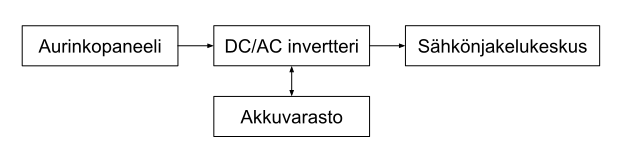
\includegraphics[width=0.75\textwidth]{figures/PV_system_components_1}
  \caption{Aurinkosähköjärjestelmän komponentit}
\end{figure}

Järjestelmä tuottaa energiaa vain tiettyyn aikaan päivästä, ja sen tuottoteho voi vaihdella hyvin nopeasti säätilasta riippuen. Kotitaloudessa nimellisteholtaan päiväsajan minimikulutusta suuremmat järjestelmät, joissa ei ole hyödynnetty kommunikaatiorajapintoja, syöttävät huipputehoaikana sähköä verkkoon päin. Kommunikaatiorajapintoja hyödyntämällä kotitaloudet voisivat hyödyntää tämän energian itse, liittämällä aurinkosähköjärjestelmän esimerkiksi kodin automaatioon. Tällöin kodista saataisiin myös energiaomavaraisempi, kun ostosähkön määrä olisi pienempi.

Järjestelmän koko, mahdolliset staattiset varjostuskohdat sekä tulevaisuuden laajentamistarpeet vaikuttavat järjestelmän suunnitteluun. Invertterin valinta vaikuttaa laite- ja asennuskustannuksiin sekä järjestelmän päivittäiseen energiantuotantoon, mutta myös järjestelmän turvallisuuteen ja suojalaitteiden tarpeeseen. Inverttereiden eri vaihtoehtoja käsitellään myöhemmin omassa kappaleessaan.

Lähes kaikki verkon käyttöpaikat ovat verkonhaltijan sähkömittarin takana. Mikäli alle 100kVA:n tehoinen tuotantolaitos sijaitsee sähkönkäyttöpaikalla, jossa on kaksisuuntainen tuntimittauslaite, ei tuotantolaitokselle tarvitse asentaa erillistä mittaria. Muussa tapauksessa tuotantolaitos vaatii erillisen sähkömittarin. Tämä johtuu käytännön syistä Yli 1MW:n järjestelmillä ei riitä tuntimittaus, vaan Fingrid vaatii tietojen lähetystiheydeksi enintään 60 sekuntia. \parencite{VJV2018}

\section{Aurinkopaneelit}
  Aurinkopaneeleiden toiminta perustuu valosähköiseen ilmiöön. Ne koostuvat suuresta määrästä sarjaan kytkettyjä aurinkokennoja, joista jokainen tuottaa tyypillisesti täydessä auringonpaisteessa hieman alle 5 W tehon noin 0,5 V jännitteellä. \parencite{Messenger}

  Aluksi, kun aurinkosähköjärjestelmät olivat pääosin verkosta irti kytkettyjä järjestelmiä, paneelit koostuivat 36 kennosta, koska tuon ajan akut olivat pääosin 12 V lyijyakkuja, joiden latausjännite vaihtelee 14–16 V välillä. Nykyään, kun aurinkosähköjärjestelmät ovat suurimmalta osin verkkoon kytkettyjä, aurinkopaneelien kennojen lukumäärä voi olla huomattavasti suurempi kuin ennen, riippuen järjestelmässä käytettävien inverttereiden sisääntulojännitteestä. \parencite{Messenger}

  Kennot ryhmitellään usein moduuleiksi, joiden kanssa rinnan kytketään ohitusdiodit. Jos kennot varjostuvat, ohitusdiodi ohittaa kyseisen moduulin, jossa varjostuneet kennot sijaitsevat, jolloin se ei aiheuta häviöitä muualla rajoittamalla muiden moduulien tai paneeleiden virtaa. Usein aurinkopaneelit ketjutetaan tarvittavan jännitteen saamiseksi, jolloin ohitusdiodien apu varjostustilanteissa on erittäin tärkeää, sillä muuten varjostuskohta rajoittaisi koko paneeliketjun virtaa. \parencite{Willeke&Weber}

  Aurinkokennojen ja -paneelien toimintakäyrinä käytetään usein virta--jännitekäyrää ja siitä johdettua teho--jännitekäyrää (engl. P--V). \begin{figure}[h]
    \centering
    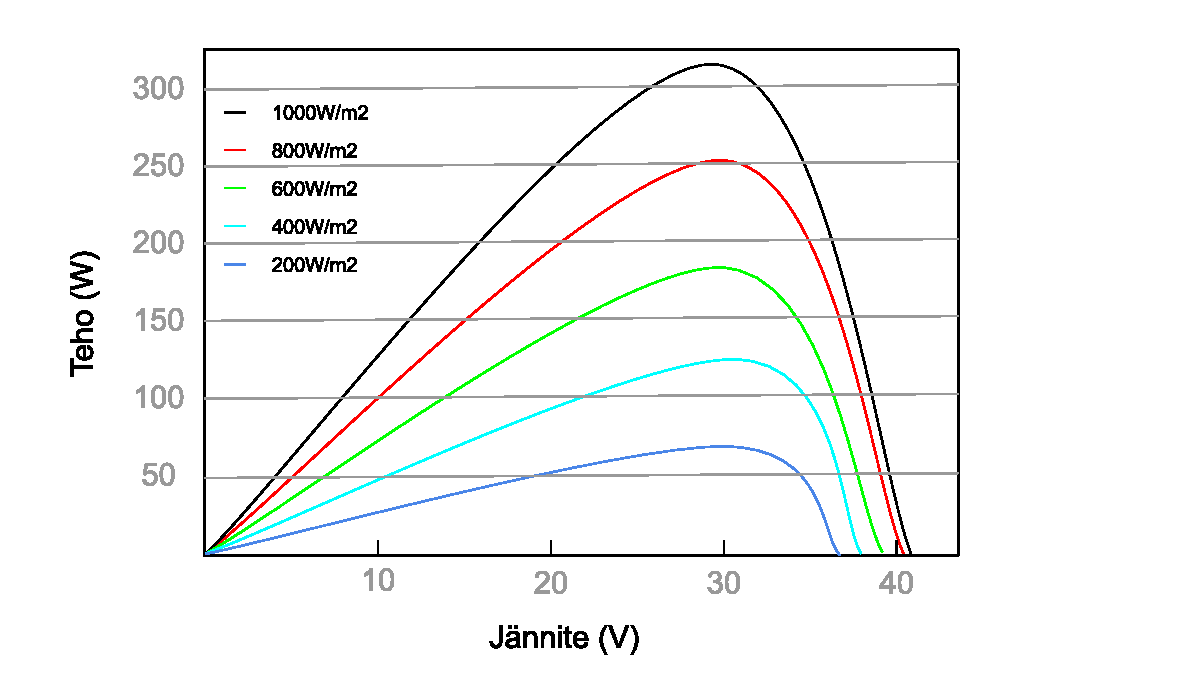
\includegraphics[width=\textwidth]{figures/pvcurve}
    \caption[Esimerkki P--V-käyrästä]{Esimerkki P--V-käyrästä. Perustuen lähteeseen \parencite{JASolar}}
  \end{figure} Kuten kuvasta 2.2 nähdään, P--V-käyrän huippukohdan sijainti vaihtelee valaisutehon mukaan. Tätä käyrän huippukohtaa kutsutaan huipputehopisteeksi (engl. Maximum Power Point, MPP). Se näyttää jännitteen, jolla saavutetaan kennon tai paneelin huipputeho kullakin valaisuteholla.

  Piirillä, jossa on sarjaan kytkettyjä aurinkopaneeleita, on jokaisella paneelilla oma paikallinen huipputehopisteensä, mutta myös koko piirillä on yhteinen globaali huipputehopiste. Globaali huipputehopiste muuttuu varjostusten ja pilvisyyden mukaan koko järjestelmän tasolla ja sitä tarkkailemalla saadaan selville, millä jännitteellä koko järjestelmästä saadaan suurin teho.

\section{Invertterit}
  Invertteri eli vaihtosuuntaaja on laite, joka muuttaa tasasähköä vaihtosähköksi. Invertterin sisääntulojännite vaihtelee käyttötarkoituksen mukaan: kaupalliseen käyttöön tai suurempiin järjestelmiin tarkoitetut laitteet toimivat korkealla, jopa \SI{1500}{\volt} jännitteellä, koska niissä on pidemmät johdotusmatkat ja suurempi määrä paneeleita kytkettynä sarjaan. Kuluttajakäytössä taas voidaan käyttää selvästi pienemmän tason jännitteitä johdotusten ollessa huomattavasti lyhyempiä ja paneeleiden määrän ollessa pienempi.

  Korkeampi jännitetaso keventää huomattavasti tarvittavaa johdotusta, kun virta voidaan pitää pienenä ja siten johtojen läpimitta pienenä. Myös häviöt pienenevät huomattavasti, koska johdoissa syntyvät häviöt kasvavat Ohmin lain
  \begin{equation}
    \textrm{P} = RI^2
  \end{equation}
  mukaan virran suhteen neliöllisenä.

  Invertteri, jolla on valmiudet huipputehopisteen seurantaan (engl. MPP Tracking, MPPT), etsii siihen kytketyn aurinkopaneeliryhmän huipputehopistettä aktiivisesti. Pisteen etsimiseen käytetään monia eri tekniikoita, mutta tämän työn kannalta niiden läpikäynti ei ole relevanttia. Jos käytetty tekniikka on liian herkkä löytämään huipputehopisteitä, se voi valita paikallisen pisteen globaalin sijaan ja aiheuttaa huomattavia tehohäviöitä väärän pisteen valinnalla. \parencite{Joshi&Arora}

  Aurinkopaneeliryhmän tehoa voidaan muuttaa kuormavastusta säätämällä. Huipputehopisteelle löytyy aina sitä vastaava ominaisvastus kaavan
  \begin{equation}
    R_{CH} = \frac{V_{MPP}}{I_{MPP}}
  \end{equation}
  mukaisesti \parencite{Joshi&Arora}, ja invertteri säätää kuormavastuksen ominaisvastuksen mukaiseen arvoon löydettyään järjestelmän huipputehopisteen mukaiset arvot kaavaan.

  Invertterit voidaan jakaa pääosin kolmeen eri tyyppiin järjestelmien topologioiden mukaan: keskusinverttereihin, mikroinverttereihin sekä ketjuinverttereihin. Keskusinvertterit ovat kaupallisissa kohteissa käytettäviä, suuritehoisia inverttereitä, kun taas mikroinvertterit ovat pääosin kuluttajakäyttöön suunnattuja laitteita. Ketjuinvertterit sijoittuvat näiden väliin ja laajan tehoskaalan vuoksi niitä voidaan käyttää molempien tyyppisissä kohteissa.

\subsection{Keskusinvertteri}
  Keskusinvertterin teho on usein hyvin suuri, yli \SI{50}{\kilo\watt}:sta jopa muutamaan megawattiin. Niitä käytetään suurissa aurinkovoimaloissa, joissa ei usein tarvitse miettiä rakennelmien tai puiden aiheuttamia varjostuksia. Tällöin asennuskustannukset pienenevät, sillä suuriin järjestelmiin riittää yksi invertteri.

  Keskusinvertterin huonoja puolia ovat järjestelmän riippuvuus yksittäisestä invertteristä sekä vain muutama huipputehopiste koko järjestelmälle. Tällöin järjestelmässä tulee suuret tehohäviöt, jos esimerkiksi pilvi kulkee osittain paneelikentän yli ja huipputehopiste määräytyy koko järjestelmälle, jolloin täysin auringossa olevien paneelien teho laskee huomattavasti. Käyttökohteiden ja suunnittelun takia tämä ei toisaalta vaikuta merkittävästi järjestelmän tuottoon.

\subsection{Mikroinvertteri}
  Mikroinvertteri on pienitehoinen vaihtosuuntaaja, joka on joko integroitu aurinkopaneelin yhteyteen tai asennettu sen välittömään läheisyyteen. Tämä tarkoittaa, että jokaiselta paneelilta voidaan säätää sen tehoa huipputehopisteen mukaiseksi. Tällöin saadaan epätasaisissa varjostustilanteissa paras mahdollinen teho, kun jokaisesta paneelista voidaan maksimoida teho. Tämä johtuu siitä, että yhden paneelin varjostuminen ei vaikuta muiden paneelien tuottoon, koska paneelit eivät ole kytketty sarjaan.

  Mikroinverttereiltä saadaan hyvin paljon tietoa, koska inverttereiden määrä järjestelmässä on suuri. Tällöin saadaan reaaliaikaisesti kuva järjestelmän toimivuudesta, ja pienetkin virhetilat voidaan korjata niiden ilmentyessä. Toisaalta inverttereiden määrä aiheuttaa haasteita tiedon koostamisessa ja tiedonsiirrossa, koska tieto ei ole välttämättä keskitetysti yhdessä paikassa sellaisenaan, vaan voi vaatia ylimääräisiä komponentteja tiedon keräämiseen.

  Kuluttajapuolen ratkaisuissa tiedonhallinta on usein toteutettu verkkokäyttöliittymällä, jolloin jokainen invertteri on liitetty erilliseen laitteeseen, joka lähettää tiedot valmistajan omaan järjestelmään tiedon koontia varten. Tästä esimerkkinä Enphasen Envoy ja Envertechin EnverBridge, jotka kommunikoivat valmistajan mikroinverttereiden kanssa PLC-väylän kautta. Sen jälkeen laite lähettää tiedot verkkoportaaliin, josta käyttäjä voi seurata paneelien tuotantoa ja järjestelmän toimivuutta. \parencite{Enphase, Envertech}

\subsection{Ketjuinvertteri}
  Ketjuinvertteriin kytketään nimensä mukaisesti sarjaan kytketyistä paneeleista muodostettuja ketjuja. Siinä on usein monta huipputehopisteen seurannan kytkentää, jolloin saadaan seurattua useita huipputehopisteitä invertteriä kohden. Invertterien teho vaihtelee muutamasta kilowatista jopa satoihin kilowatteihin, jolloin sitä voidaan käyttää hyvin erikokoisissa järjestelmissä.

  Teholuokaltaan pienet ketjuinvertterit on suunniteltu käyttäjäystävällisyyshuomioiden, ja esimerkiksi SMA:n ja Huawein invertterit sisältävät integraation valmistajien taustajärjestelmiin. SMA on toteuttanut tämän integraation valmiina laitteelle, kun taas osa Huawein inverttereistä vaatii sovittimen Ethernet-portin, WLAN:in tai matkapuhelinverkon käyttämiseen datasiirrossa.

  SMA:n invertterit käyttävät lisäksi SunSpec Alliancen SunSpec Modbus -standardia, joka toimii Ethernet-verkon välityksellä. Muut standardia hyödyntävät valmistajat voivat kommunikoida suoraan SMAn inverttereiden kanssa standardoinnin takia. Huawei käyttää myös Modbus-protokollaa, mutta se ei ole SunSpec Alliancen standardoima. Tämä tarkoittaa, että Huawein kanssa kommunikoitaessa sille on räätälöitävä ohjelmistoa datan lukemiseksi. \parencite{SMAManual, Huawei}

  Modbusin hyödyntäminen mahdollistaa muiden valmistajien tuotteiden kommunikaation inverttereiden kanssa. Yhteinen standardi helpottaa suurissa järjestelmissä eri valmistajien tuotteiden yhteensopivuuden kanssa, mutta ylipäätään Modbusin käyttö antaa mahdollisuuden kolmannen osapuolen tuotteiden liittämiseen.

\section{Järjestelmien tuotto-ominaisuudet}
  Aurinkosähköjärjestelmät ovat sähköntuottajina teholtaan nopeasti muuttuvia. Niiden tuoton ennustaminen on jokseenkin mahdollista päivätasolla, mutta tuntitehon ennustaminen sääennusteen perusteella on jo haastavaa. Toisaalta, kun tuotannon määrä verkossa kasvaa, eri sijainnissa olevat järjestelmät tasaavat näitä tuotannon vaihteluita ja suuressa kuvassa niiden kokonaistuotantokäyrä ''pehmenee''. Tätä on tutkittu tuulivoiman osalta, joka sähköntuottajana on aurinkosähkön kanssa samankaltainen. \parencite{FluctuationIssues}
  
  Nykyisellä keskitettyyn sähköntuotantoon rakennetulla verkolla aurinkosähköjärjestelmät tuovat haasteita, sillä pientuotantoa lisätessä johtolähtöjen jännitetasot nousevat ja verkon suojaustoimintoja voidaan joutua päivittämään. Esimerkiksi mikrotuotanto voi aiheuttaa vikavirtasuojauksen virhelaukaisun, mikäli tuotanto on lähellä muuntajan kiskoa ja se alkaa syöttämään läheisen lähdön vikatilanteessa vikavirtaa kiskoa kohti. Tällöin terveessä lähdössä tapahtuu virhelaukaisu. \parencite{Mikrotuotanto}
  
  Aurinkosähkön osuuden kasvaminen sähköntuotannossa lisää säädettävän tuotantokapasiteetin tarvetta sähkömarkkinoilla. Päivän aikana nettotehonmuutos on suuri, kun aurinkosähköjärjestelmät alkavat tuottaa sähköä samalla, kun kysyntä laskee ihmisten lähtiessä töihin. Vastaavasti sama tapahtuu illalla kun ihmiset palaavat töistä ja järjestelmän tuottoteho laskee. Tätä ilmiötä kuvaa niin sanottu ''duck''-käyrä, joka nähdään kuvassa 2.3. \begin{figure}
    \centering
    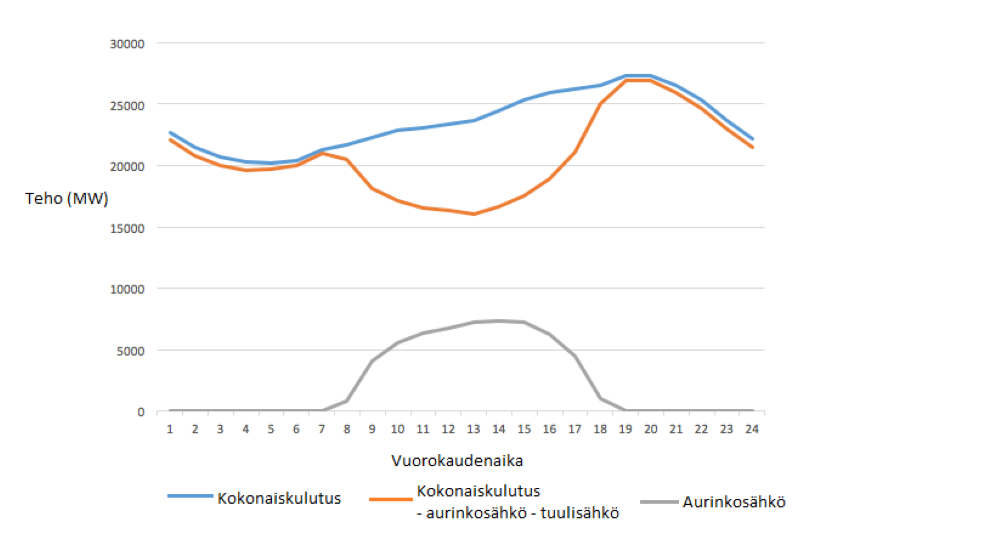
\includegraphics[width=1.1\textwidth]{figures/Duck_curve.png}
    \caption{''Duck''-käyrä}
  \end{figure} Se kuvaa säädettävän energiatuotannon keskimääräistä hetkellistä tuotantotehoa vuorokauden aikana. \parencite{duckCurve}

  Tuotantokapasiteetin tarvetta voidaan helpottaa energiavarastojen avulla, jolloin päivän energiantuotantoa saadaan siirrettyä illan huippukuormituksen ajalle. Energiavarastot tasaavat myös aurinkosähkön tuotannon ailahtelevuutta. Ongelmana energiavarastojen määrän lisääntymisessä on kuitenkin niiden korkea hankintahinta ja niistä saatavat hyödyt.

  Yksittäiselle kuluttajalle energiavarastoista saatavat hyödyt tulevat tuotetun sähkön hyödyntämisestä kalliimman sähkönhinnan aikaan, sillä kuluttajan saama tuotto myydystä sähköstä on pienempi kuin itse kulutetun energian hinta. Lisäksi tuottaja voi haluta kodistaan enemmän energiaomavaraisen ja käyttää tuotetun sähkön kokonaan itse. Mikäli kuluttajalla ei ole kulutusjoustoon soveltuvia laitteita, voi se hyödyntää energiavarastoa tuotetun sähkön hyödyntämiseen tuotantoajan ulkopuolella.
  
  Tuottajalla on taas useampi syy energiavarastojen hyödyntämiseen. Matala sähköstä saatava markkinahinta on myös tuottajalla syy hyödyntää energiavarastoa, varsinkin jos hinta on tuotantohuipun aikaan matala. Verkkokoodi määrittelee tuotantolaitoksien sähköverkkoon liittämisvaatimukset. Tulevaisuudessa se voi pakottaa tuotantolaitokset investoimaan energiavarastoon sähköverkon vakauden ja jännitteen laadun ylläpitämiseksi. Vaikka verkkokoodi ei pakottaisi investoimaan energiavarastoon, voi se olla kannattavaa, jos verkonhaltija joutuisi vahvistamaan verkkoa ja liittyjän kustannukset nousisivat muuten. Tariffihinnoittelun muuttuminen tulevaisuudessa tehopohjaiseksi kannustaa yrityksiä investoimaan myös energiavarastoihin, sillä niillä voidaan loiventaa kulutushuippua, jolloin tariffimaksu pienenee.


\chapter{Lämpöpumput sähkön käyttäjinä}
\label{ch:pumput_sahkon_kayttajina}
Tässä kappaleessa perehdytään lämpöpumpun toimintaperiaatteeseen ja siihen miten se käyttäytyy sähkön käyttäjänä. Lämpöpumpun vaikutukset sähköverkkoon riippuvat lämpöpumpun teknisistä ratkaisuista kuten tehon mitoituksesta ja moottorin syöttötavasta. Myös verkon ominaisuudet vaikuttavat pumpun käyttöön.

Lämpöpumppuja käytetään pääasiassa kiinteistöjen lämmitykseen ja viilennykseen. Muita kohteita ovat esimerkiksi teollisuus, jossa lämpöpumppujen avulla voidaan tuottaa prosessien tarpesiin lämpöä hyödyntämällä hukkalämpöä, tai kaukolämmöntuotanto.\parencite{Setala, katriVala} Lämpöpumppu saattaa olla kiinteistön ainoa lämmitysmuoto, tai se saattaa toimia toisten lämmitysjärjestelmien rinnalla. Lämpöpumpuilla voidaan korvata vanha järjestelmä, millä on vaikutusta kiinteistön lämmityksen aiheuttamaan sähkönkulutuksen luonteeseen. Esimerkiksi korvattaessa vanha öljy- tai puulämmitys lämpöpumpulla, sähkönkulutus kasvaa. Korvatessa suora sähkölämmitys lämpöpumpulla, muuttuu taas sähkön kulutuksen luonne. Lämpöpumppu käyttää saman lämmön tuottamiseen vähemmän sähköenergiaa, mutta huipputehot saattavat olla suurempia.

\section{Lämpöpumpun toimintaperiaate}
  Lämpöpumpun eli jäähdytyskoneen toimintaperiaate on käänteinen lämpövoimakoneelle. Lämpöpumppu siirtää lämpöenergiaa viileämmästä ympäristöstä lämpimämpään.\parencite{DincerRosen}

  Lämpöpumpun perusrakenne koostuu kompressorista, lauhduttimesta, paisuntaventtiilistä ja höyrystimestä, joiden välillä kiertää kylmäaine. Järjestelmä on kuvattu kuvassa \ref{fig:hptp}. Matalassa paineessa oleva kylmäaine höyrystyy viileämmässä tilassa sijaitsevassa höyrystimessä ja vastaanottaa lämpöenergiaa. Höyrystynyt kylmäaine johdetaan lauhduttimeen ja sen paine nostetaan kompressorin avulla korkeammaksi, jolloin sen lämpötila nousee. Korkeassa paineessa ja lämpötilassa oleva kylmäaine luovuttaa lämpöenergiaa lauhduttimen välityksellä lämpimään ympäristöön, jolloin osa siitä nesteytyy. Nesteytynyt kylmäaine virtaa paisuntaventtiilin kautta takaisin höyrystimeen. Paisuntaventtiilissä kylmäaineen paine ja täten myös lämpötila laskevat.\parencite{DincerRosen}

  Höyrystimessä lämpöenergiaa siirtyy kylmäaineeseen ympäristöstä. Lämmön kuljettaminen ympäristöstä höyrystimelle voidaan toteuttaa erilaisilla tavoilla. Suomessa yleisin tapa on käyttää ilmapuhallinta \parencite{sulpu}, joka puhaltaa ulkoilmaa höyrystimen lävitse ja jäähdyttää sitä. Tällöin kyseessä on ilmalämpöpumppu. Toinen yleinen vaihtoehto on käyttää maahan kaivettavaa tai kallioon porattavaa lämmönkeruuputkistoa. Tällaista lämpöpumppua kutsutaan maalämpöpumpuksi. Eri sovelluskohteissa käytetään myös lukuisia muitakin lämmönlähteitä kuten ilmanvaihdon poistoilmaa, viemärivettä, lauhdevettä tai vesistöä.\parencite{DincerRosen}

  Lauhduttimessa kylmäaineen luovuttama lämpöenergia siirretään sovelluskohteesta riippuen esimerkiksi käyttöveteen, lämmitysjärjestelmän vesikiertoon tai suoraan huoneilmaan. Teollisuudessa tuotettua energiaa voidaan käyttää esimerkiksi erilaisissa prosesseissa\parencite{Setala}. Sovelluskohde määrää lauhduttimelta vaadittavan lämpötilan. Järjestelmiä saatetaan kutsua erilaisilla nimillä riippuen siitä, mihin tuotettua energiaa käytetään. Mikäli tuotetulla energialla lämmitetään käyttövettä tai lämmitysjärjestelmän kiertovettä, kutsutaan laitetta Ilma--vesilämpöpumpuksi. \parencite{sulpu}

  Lämpöpumpun lämpökerroin, eli COP\footnote{Coefficient Of Performance} määritellään lämpöpumpun tuottaman lämpötehon ja sen kuluttaman sähkötehon suhteena
  \begin{equation}
      \textrm{COP} = \frac{\dot{Q}}{\dot{P}}
  \end{equation}
  Normaali lämpöpumppujen lämpökerroin vaihtelee välillä 2--5. Lämpökerroin ja sen vaihtelu riippuvat paljolti lämmön lähteestä: maalämpöpumpuilla on yleensä korkeampi lämpökerroin kuin ilmalämpöpumpuilla.\parencite{DincerRosen} Myös haluttu lauhduttimen lämpötila vaikkuttaa lämpökertoimeen. Mitä korkeampi lämpötila lauhduttimelle halutaan sen matalampi pumpun lämpökerroin on. \parencite[kuva 7.6]{DincerRosen}

  \begin{figure}
    \centering
    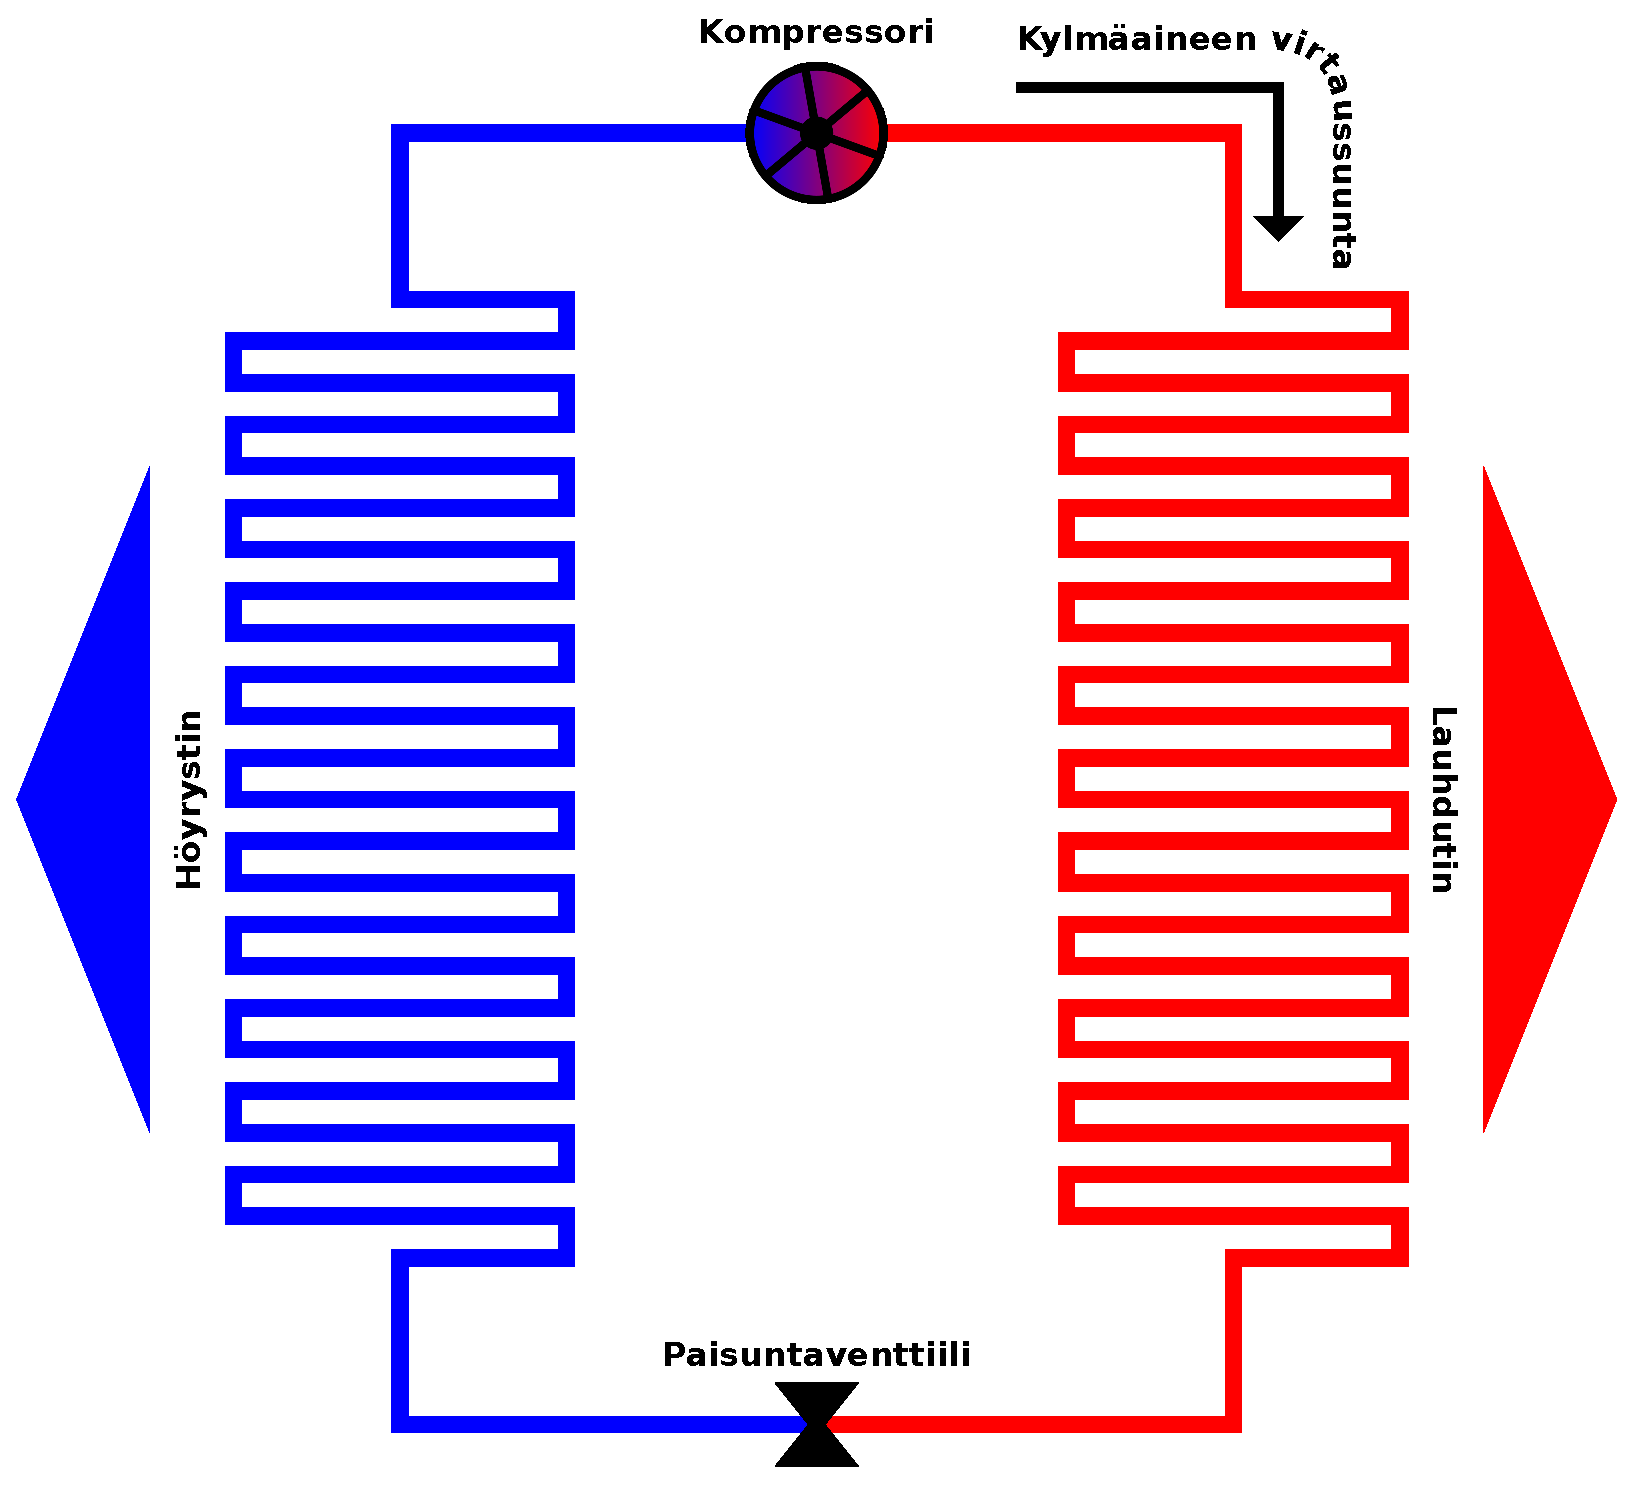
\includegraphics[width=0.5\textwidth]{figures/hp}
    \caption{Lämpöpumpun toimintaperiaate}
    \label{fig:hptp}
  \end{figure}

  Lämpöpumput käyttävät sähköenergiaa lämmön siirtämiseen viileämmästä lämpövarastosta lämpimämpään. Käytetystä sähköenergiasta valtaosa kuluu paineen tuottamiseen kompressorilla, mikä ylläpitää energiaa tuottavaa työkiertoa. Kompressorin lisäksi sähköä kuluu pienempiä määriä vaikkapa lämpöpumpun ohjaukseen, lämmitysjärjestelmän kiertovesipumpun käyttämiseen tai puhaltimen käyttämiseen. Mikäli lämpöpumpun teho on mitoitettu pienemmäksi kuin suurin vaadittu lämmitysteho\footnote{osatehomitoitus}, voidaan tehojen erotus tuottaa tarvittaessa lämpöpumpun yhteyteen asennettavilla sähkövastuksilla. Tällainen ratkaisu lisää huomattavasti järjestelmän sähkönkulutusta suurimman lämmitystarpeen aikana, jolloin sähköä käytetään muutenkin enemmän. Järjestelmän käyttäminen viilentämiseen taas lisää energian kulutusta, silloin kun sähkön käyttö on muuten todennäköisesti vähäisempää.

  Lämpöpumpuissa kompressorin pyörittämiseen käytetään sähkömoottoria. Vanhemmissa lämpöpumpuissa moottori on useimmiten verkkojännitteeseen kytketty oikosulkumoottori, joka voidaan tarvittaessa varustaa käynnistyksen ohjauksella eli pehmokäynnistimellä. Nykyaikaisemmassa ratkaisuissa oikosulkumoottoria käytetään taajuusmuuttajan avulla.

\section{Oikosulkumoottori}
  Yleisin tapa pyörittää lämpöpumpun kompressoria on käyttää suoraan verkkojännitteeseen kytkettyä oikosulkumoottoria. Kompressorin tehoa ei voida säädellä, vaan käydessään se tuottaa aina vakiotehon. Tällaisen lämpöpumpun tehoa säädetään kytkemällä kompressoria päälle ja pois. Kompressori kytkeytyy päälle, kun lämmitettävän kohteen, esimerkiksi lämminvesivaraajan tai sisäilman, lämpötila laskee tietyn rajan alapuolelle. Kun lämmitettävän kohteen lämpötila on noussut tarpeeksi, sammutetaan kompressori.

  Tärkeimmät kompressorin käyntijaksojen pituuteen vaikuttavat tekijät ovat lämmitettävän kohteen haluttu lämpötila ja lämpöenergian tarve, lämmönlähteen lämpötila ja kompressorin teho. Kotitalousköytössä kompressoreiden tehot ovat yleensä muutamia kilowatteja\footnote{etsi tarkempi tieto}.

  Mikäli oikosulkumoottorin käynnistysvirtaa ei mitenkään rajoiteta, on se tyypillisesti 6 -- 8 kertainen moottorin nimellisvirtaan nähden. Täten myös moottorin sähköverkosta käynnistyessään ottama teho on suuri.\parencite{pehmokaynnistinopas} Käynnistyksen jälkeen moottorin ottama virta ja teho laskevat kompressorin ottotehon määräämään arvoon.

  Oikosulkumoottorien suuret käynnistysvirrat näkyvät tehopiikkeinä myös sähköverkon puolella. Mikäli samassa muuntopiirissä on useampia lämpöpumppuja tai alhainen jännitejäykkyys, saattavat pumput aiheuttaa jännitetason vaihteluita. Alhaisen jännitejäykkyyden omaavissa verkoissa jo lämpöpumppujen normaalit käynnistykset saattavat aihetuttaa jännitetasonvaihteluita, jotka ilmenevät esimerkiksi välkyntänä\parencite{SFSEN50160}. Sähkökatkojen jälkeen kytkettäessä jännitettä takaisin, useat lämpöpumput saattavat käynnistyä samaan aikaan lämmittämään viilentyneitä lämmityskohteitaan. Tämä saattaa aiheuttaa lyhytaikaisen jännitteen aleneman. Mikäli jännitteenaleneman jälkeinen jäännösjännite on alle \SI{90}{\percent} järjestelmän nimellisjännitteestä, kutsutaan sitä jännitekuopaksi\parencite{SFSEN50160}.

  Oikosulkumoottoreiden käämityksistä johtuen ne ovat induktiivista kuormaa ja täten kuluttavat loistehoa. Mikäli moottoreiden kuluttamaa loistehoa ei kompensoida tuottamalla sitä paikallisesti, näyttäytyy lämpöpumppu sähköverkkoon induktiivisena kuormana. Induktiivisen kuorman kuluttama loisteho lisää häviöitä sähköverkossa ja loistehon kompensoinnin tarvertta verkkotasolla.\parencite{pakonen} \marginpar{onko kompensointia?}


\section{Oikosulkumoottori pehmokäynnistimellä}
  Lämpöpumpun käynnistyessään ottamaa virtapiikkiä voidaan pienentää tai se voidaan poistaa kokonaan pehmokäynnistimellä. Pehmokäynnistimen toiminta perustuu tyristoreihin, joilla säädellään moottorin kokemaa jännitettä. Alussa tyristorit johtavat vain hyvin pienen osan jännitteen jaksonajasta ja moottori alkaa tuottamaan momenttia. Vähitellen kasvatetaan tyristoreiden läpi päästettyä jännitteen osuutta, kunnes tyristorit ovat täysin johtavassa tilassa. Kun moottori on saavuttanut käyntinopeutensa, eivät tyristorit enää rajoita virtaa, ja ne voidaan esimerkiksi ohittaa kytkimellä tehohäviöiden pienentämiseksi.\parencite{pehmokaynnistinopas}

  Pehmokäynnistimen käyttö poistaa lämpöpumppujen käynnistysvirtapiikkien aiheuttaman ongelman. Pehmokäynnistimellä ei voida kuitenkaan järkevästi vaikuttaa moottorin käydessään ottamaan tehoon tai sen tuottamaan energiamäärään.

\section{Taajuusmuuttajakäytöt}
  Nykyaikainen ratkaisu lämpöpumpujen kompressorien käyttämiseen on taajuusmuuttaja. Taajuusmuuttaja koostuu tasasuuntaajasta ja ohjatusta vaihtosuuntaajasta, jolla saadaan tuotettua halutun suuruista ja taajuista vaihtojännitettä. Käynnistettäessä kompressoria aloitetaan moottorin syöttäminen matalataajuisella vaihtojännitteellä. Moottorin käyntinopeuden noustessa kohti haluttua arvoa, nostetaan samalla jännitteen taajuutta niin, että verkosta otettu teho pysyy suurin piirtein vakiona pyörimisnopeudesta riippumatta.

  Taajuusmuuttajan käytöllä saavutetaan useita hyötyjä. Käynnistysvirtapiikkien poistamisen lisäksi taajuusmuuttajalla voidaan myöskin säädellä kompressorin tuottamaa tehoa. Tehon säätäminen mahdollistaa pidemmät käyntijaksot ja tasaisemman tehonkulutuksen, mutta ei kuitenkaan vähennä lämpöpumpusta saatavaa maksimitehoa. Pienempien energiamäärien tuottaminen toteutetaan pienentämällä kompressorin käyntinopeutta, jolloin lämpöpumppua ei tarvitse käyttää useissa lyhyemmissä käyntijaksoissa.

  Verkon näkökulmasta taajuusmuuttaja näyttäytyy eri tavoilla riippuen siitä, miten siinä on totetutettu vaihtovirran tasasuuntaus. Perinteisissä ja halvemmissa taajuusmuuttajissa tasasuuntaus on toteutettu diodisillalla. Diodisilta aiheuttaa sisääntulevan virran säröytymistä ja sitä kautta myöskin jännitehäiriöitä verkkoon. Myöskään lämpöpumpun tehokertoimen säätäminen ei onnistu. Diodisiltaa parempi ratkaisu on verkkovaihtosuuntaaja, jonka ottama virta voidaan säätää lähes sinimuotoiseksi, jolloin virtasärön syntyminen voidaan ehkäistä. Verkkovaihtosuuntaajan tehokerrointa voidaan myöskin säätää, jolloin sitä voidaan käyttää loistehotasapainon ylläpitämiseen. Mikäli lämpöpumppua syöttävä taajuusmuuttaja on säädetty niin, että se näyttäytyy verkkoon lähes resistiivisenä kuormana se osaltaan vähentää verkon kuormitusta ja laskee jännitehäviöitä. Taajuusmuuttajan verkkoon aiheuttamat jännitehäiriöt riippuvat paljon taajuusmuuttajasta, sen laadusta ja koosta. \parencite{koskenjoki}

\section{Resistiivinen kuorma}
  Moottorikuormien lisäksi lämpöpumppujen yhteyteen asennetaan usein lämpövastuksia. Mikäli kyseessä on osatehomitoitettu lämpöpumppu, vastuksia käytetään suurimman energiatarpeen aikana, jolloin lämpöpumppu itsessään ei kykene tuottamaan kaikkea tarvittavaa energiaa. Lämpövastuksia käytetään myöskin höyrystimeen kertyneen jään ja huurteen poistoon.

  Lämpöpumpuissa kuluu sähköä myös muihin tarkoituksiin kuin suoraan energiantuotantoon. Automatiikan, ohjauksen ja sisä- ja ulkoyksiköiden puhaltimien kuluttama energia on kuitenkin vähäistä verrattuna muuhun energiankulutukseen


\chapter{Rajapinnat -- eri abstraktiotasot}
\label{ch:rajapinat}
Rajapinnat mahdollistavat tiedonvaihdon eri järjestelmien ja toimijoiden välillä. Ne voivat olla standardissa määriteltyjä, eri abstraktiotasoille ja osittain toistensa päälle rakentuvia, tai hyvin suljettuja laitteen valmistajan kehittämiä. Lisäksi yhtenä rajapintana lämpöpumpuille ja aurinkoinverttereille voidaan ajatella AMI-mittareita.

Valmistajan tarjoamat pilvipalvelut toimivat rajapintana järjestelmän etähallintaan ja -monitorointiin omistajalle. Myös valmistaja itse voi hyödyntää tätä rajapintaa esimerkiksi selvittämällä etänä laitteistovikaa tai keräämällä tilastoja järjestelmän toimivuudesta. Teknisesti ajatellen pilvipalvelu on kuitenkin standardoimaton, valmistajan itse kehittämä, joten tekninen toteutus on piilotettu. Tämän vuoksi tässä kappaleessa ei perehdytä tarkemmin pilvipalveluun, vaan se esitellään vain yleisesti.

Kaikkein matalimman abstraktiotason rajapintoja eli fyysisiä liitäntöjä tai sarjaliikenneprotokollia ei tässä työssä käsitellä tarkemmin. Tässä kappaleessa on kuvattu eri standardeissa määriteltyjen rajapintojen toimintaa ja käyttötarkoituksia. Lisäksi tarkastellaan myös \gls{AMI}-mittareita rajapintana.

\section{Modbus}

  Modbus on automaatiossa käytetty palvelin--asiakas-mallin viestintäprotokolla. Sen on alun perin kehittänyt vuonna 1979 yritys nimeltään Modicon käytettäväksi valmistamiensa ohjelmoitavien logiikoiden eli \Gls{plc}:den väliseen viestintään. Nykyisin Modicon on osa ranskalaista Schneider Electriciä. Koska standardi on julkaistu avoimesti kaikkien käytettäväksi ja se on verrattain yksinkertainen, on se saavuttanut johtavan aseman teollisuudessa. Yleisimmille ohjelmointikielille on saatavilla Modbus-standardin toteuttavat kirjastot, joiden avulla voidaan ohjelmallisesti ohjata laitteita. Laajan levinneisyyden ansiosta Modbus soveltuu monien eri valmistajien laitteiden järjestelmien kanssa käytettäväksi. Teollisuuden lisäksi protokollaa käytetään myös talo- ja kiinteistöautomaatiossa.\parencite{sousaPortugal, modbusAppSpec, modbusOrg}

  Vuonna 2004 Schneider Electric siirsi standardin hallinnan voittoa tavoittelemattomalle Modbus-järjestölle\footnote{Modbus Organization, Inc}. Järjestön muodostavat automaatiolaitteita valmistavat yritykset ja yksittäiset henkilöt. Sen tehtäviin kuuluu ylläpitää ja kehittää Modbus-standardia ja siihen liittyviä documentteja sekä toimia etujärjestönä edistäen modbusin käyttöä. Modbusiin liittyvien dokumenttien ja julkaisujen avulla edistetään eri valmistajien järjestelmien välistä kommunikaatiota ja helpotetaan niiden integraatioita toisiinsa.  \parencite{modbusOrg}

  \subsection{viestintä ja tietomalli}

  Modbus-protokollan toiminta perustuu palvelinlaitteella sijaitsevien muistialueiden lukemiseen ja kirjoittamiseen kuvassa \ref{fig:c_s} kuvatun asiakas--palvelin-mallin (client--server model, ennen tunnettu termillä master--slave model) mukaan.  Lukemalla tietoja asiakaslaite kykenee seuraamaan palvelinlaitteen tilaa ja kirjoittamalla ohjaamaan sen toimintaa. Tietojen lukeminen ja kirjoittaminen tapahtuu protokollan määrittämien kysely, vastaus- ja virheviestien perusteella.\parencite{modbusAppSpec}

  \begin{figure}[h]
    \centering
    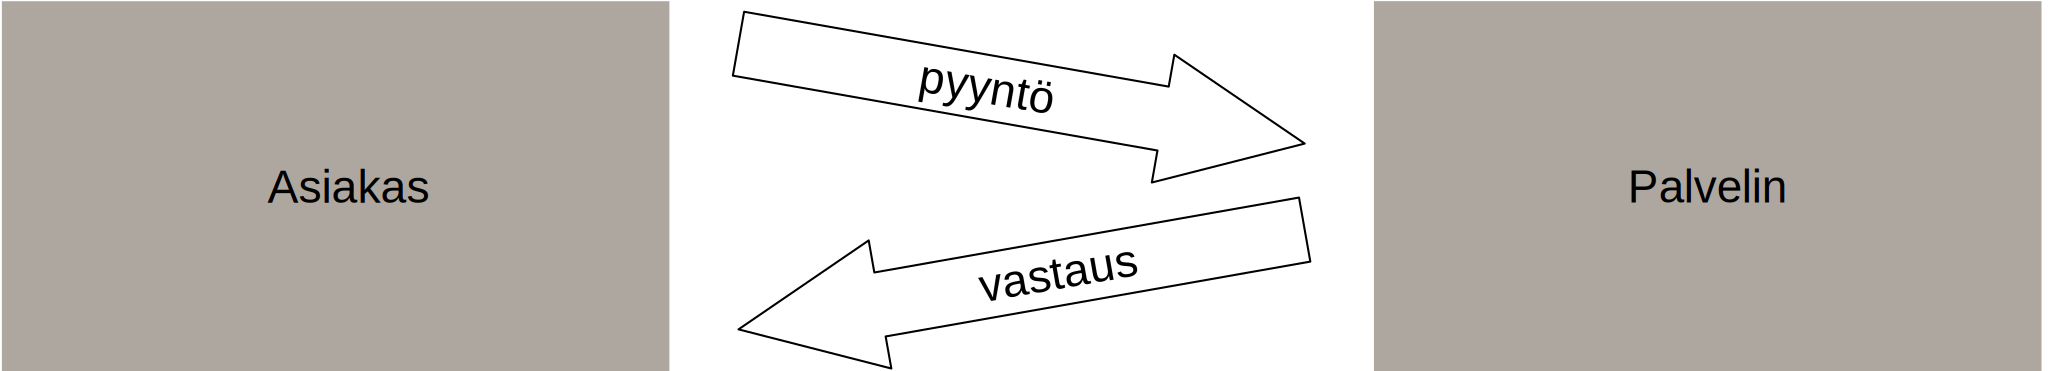
\includegraphics[width=1\textwidth]{figures/client_server}
    \caption[asiakas--palvelin-malli]{Asiakas--palvelin-malli.  Perustuen lähteeseen \parencite{modbusAppSpec}}
    \label{fig:c_s}
  \end{figure}

  Modbus-verkko muodostuu yhdestä asiakkaasta, ja yhdestä tai useammasta palvelimesta. Palvelimet yksilöidään kokonaislukuosoitteella väliltä 1--247, mikä rajoittaa samaan verkkoon kytkettyjen latteiden määrää.  Protokolla rajoittaa kommunikointia niin, että kyselyitä lähettää vain asiakaslaite palvelinlaitteiden ainoastaan vastatessa niille osoitettuihin kyselyihin.\parencite{modbusSerialSpec} Tästä johtuen palvelinlaitteen eivät kykene itsenäisesti raportoimaan mahdollisesta virhetilanteesta tai tapahtumasta, vaan asiakaslaitteiden on jatkuvasti tehtävä kyselyitä pysyäkseen ajan tasalla. Tämä Modbusin ominaisuus vähentää sen käyttökelpoisuutta, varsinkin, mikäli kommunikointiresurssit ovat rajalliset.

  Modbus-protokolla määrittelee lähetettäville kyselyille kaksi eri muotoa: täsmälähetys (unicast) ja monilähetys (multicast). Täsmälähetys osoitetaan tietylle palvelimelle ja vastaanotettuaan sen palvelin toimii sen mukaisesti. Monilähetys taas lähetetään osoitteella 0, jolloin kaikki palvelimet reagoivat kyselyyn.\parencite{modbusSerialSpec} Kerrallaan vain yksi laite verkossa voi toimia asiakkaana muiden toimiessa palvelimina. Tästä huolimatta yksittäinen laite voi kuitenkin toimia sekä palvelimena, että asiakkaana, kunhan tämä tapahtuu erillisissä verkoissa.\parencite{DincerRosen}

  Modbus-protokollan tietomalli koostuu palvelinlaitteella sijaitsevista muistialueista, jotka on jaettu taulukoihin. Pääasialliset neljä muistialuetaulukkoa on kuvattu taulukossa \ref{taulukot}. Taulukoiden nimeäminen suomen kiellellä on haastavaa, joten se jätetään tekemättä.
  \begin{table}[h]
    \centering
    \caption[Modbus muistialuetaulukot.]{Modbus muistialuetaulukot. Perustuu lähteeseen \parencite{modbusAppSpec}.}
    \begin{tabular}{|l|l|l|}
      \hline
      \rowcolor{gray} taulukon tyyppi         & datatyyppi      & asiakkaan oikeudet  \\ \hline
      \cellcolor{lightgray}Discretes Input    & 1 bitti          & vain luku           \\ \hline
      \cellcolor{lightgray}Coils              & 1 bitti          & luku/kirjoitus      \\ \hline
      \cellcolor{lightgray}Input Registers    & 16-bittinen sana & vain luku           \\ \hline
      \cellcolor{lightgray}Holding Registers  & 16-bittinen sana & luku/kirjoitus      \\ \hline
    \end{tabular}
    \label{taulukot}
  \end{table}
  1-bittisiä muistipaikkoja voidaan käyttää esimerkiksi päälläolotietojen välittämiseen, kun taas kahden tavun mittaisia muistipaikkoja voidaan käyttää esimerkiksi mitattujen arvojen ilmoittamiseen. Protokolla ei kuitenkaan määritä miten muistipaikkoja kuuluu käyttää, vaan tämä jätetään sovelluksen tekijän päätettäväksi. Kussakin taulukossa on 65536 erillistä osoitetta, joihin dataa voi tallentaa. Datan käsittely tapahtuu joko yksittäisen osoitteen perusteella tai sitten useampi perättäinen osoite kerrallaan.\parencite{modbusAppSpec}

  \subsection{Application data unit}

    Laitteissa toimivien sovellusten väliseen tiedonsiirtoon käytetään \gls{PDU}:a (Application Data Unit), joka koostuu funktiokoodista ja operaatioon tarvittavasta datasta. \gls{PDU}:ja on kolmenlaisia, ja ne on esitetty taulukossa \ref{pdu}.
    \begin{table}[h]
      \centering
      \caption[\gls{PDU}-tyypit.]{\gls{PDU}-tyypit. Perustuu lähteeseen \parencite{modbusAppSpec}.}
      \begin{tabular}{ccl}
        \cellcolor{green}Funktiokoodi (F)              & \cellcolor{green}Kyselyn data    & Kysely-PDU   \\
                                                       &                                  &              \\
        \cellcolor{green}Funktiokoodi (F)              & \cellcolor{green}Vastauksen data & Vastaus-PDU  \\
                                                       &                                  &              \\
        \cellcolor{red}Poikkeusfunktiokoodi (F + 0x80) & \cellcolor{red}Poikkeuskoodi     & Poikkeus-PDU \\
      \end{tabular}
      \label{pdu}
    \end{table}

    \gls{PDU}:n alun muodostaa funktiokoodi, joka on joko Modbus-protokollan tai käyttäjän määrittämä funktio. ADU:n loppuosa koostuu mahdollisesta datasta, jota palvelin tarvitsee suorittaakseen halutun toiminnon. Vastaus-PDU:hun tulee sama funktiokoodi kuin kysely-PDU:hun. Mikäli palvelin päätyy virhetilanteeseen, joko virheellisen kysely-PDU:n tai sisäisen virheen takia, vastaa se asiakkaalle poikkeus-PDU:lla, joka muodostuu funktiokoodista, johon on liitetty heksakoodi 0x80, ja poikkeuskoodista.\parencite{modbusAppSpec} Funktiokoodeista käytetyimmät liittyvät yksittäisten muistipaikkojen lukemiseen ja kirjoittamiseen\parencite{DincerRosen}. Lista yleisistä funktio- ja poikkeuskoodeista löytyy liitteestä \ref{app:modbus_funktio_koodit}.


  \subsection{protokollan rakenne}

    Modbus-protokollasta on toteutettu muutamia eri versioita:
    \begin{itemize}
      \item sarjaväyläversio eli Modbus Serial, joka muodostuu kahdesta muunnelmasta:
      \begin{itemize}
        \item Modbus \gls{RTU} ja
        \item Modbus ASCII,
      \end{itemize}
      \item Modbus TCP/IP ja
      \item Modbus Plus.
      \parencite{modbusAppSpec}
    \end{itemize}
    Edellisistä Modbus Plus on Schneider Electricin hallinnoima, eikä se ole avoimesti saatavilla. Modbus Plus on oma Modbusista eroava standardinsa, jota ei tässä käsitellä enempää.\parencite{seCom}

    Taulukossa \ref{rakenne} on Modbus-protokollaperhettä verrattu \gls{OSI}-malliin. Modbus-protokollan ylempi kerros, eli \gls{MBAP} sijoittuu \gls{OSI}-mallissa kerroseen 7, eli sovelluskerrokseen. \gls{MBAP}:n toimintaa on esitelty edellisessä kappaleissa. Sarjaväyläversiossa alempi kerros sijoittuu \gls{OSI}-mallissa kerrokseen 2 ja Modbus TCP/IP:n tapauksessa kerrokseen 5\footnote{\gls{OSI}-mallin teoreettisesta luonteesta johtuen tästä voinee esittää eroavia mielipiteitä.}.
    \begin{table}
      \centering
      \caption[Modbus-protokollan rakenne ja \gls{OSI}-malli]{Modbus-protokollan rakenne ja sen sovitus \gls{OSI}-malliin. Modbus-protokollaperhe sinisellä. Perustuu lähteisiin \parencite{osi, modbusSerialSpec, modbusTCPIPSpec}.}
      \begin{tabular}{|c|c|ccc}
        \cline{1-2}
        \multicolumn{2}{|c|}{OSI-mali}                                               & \multicolumn{3}{c}{}                                                                                                                                                                           \\ \hline
        \multicolumn{1}{|l|}{}                    &                                  & \multicolumn{3}{c|}{\cellcolor{yellow}SunSpec}                                                                                                                                                 \\ \cline{3-5}
        \multicolumn{1}{|l|}{7}                   & sovelluskerros                   & \multicolumn{3}{c|}{\cellcolor{blue}MBAP (Modbus-viestintäprotokolla)}                                                                                                                         \\ \hline
        6                                         & esityskerros                     &                                                         &                                                           & \multicolumn{1}{c|}{}                                                    \\ \cline{1-2} \cline{5-5}
        5                                         & istuntokerros                    &                                                         & \multicolumn{1}{c|}{}                                     & \multicolumn{1}{c|}{\cellcolor{blue}Modbus-\gls{TCP}}                    \\ \cline{1-2} \cline{5-5}
        4                                         & kuljetuskerros                   &                                                         & \multicolumn{1}{c|}{}                                     & \multicolumn{1}{c|}{\gls{TCP}}                                           \\ \cline{1-2} \cline{5-5}
        3                                         & verkkokerros                     &                                                         & \multicolumn{1}{c|}{}                                     & \multicolumn{1}{c|}{IP}                                                  \\ \hline
        2                                         & siirtokerros                     & \multicolumn{1}{c|}{\cellcolor{blue}Modbus-RTU}         & \multicolumn{1}{c|}{\cellcolor{blue}Modbus-ASCII}         & \multicolumn{1}{c|}{Ethernet, \dots}                                     \\ \hline
        1                                         & fyysinen kerros                  & \multicolumn{2}{c|}{RS-232 / RS-485}                                                                                & \multicolumn{1}{c|}{Ethernet, \dots}                                     \\ \hline
      \end{tabular}
      \label{rakenne}
    \end{table}

    \gls{MBAP} on kaikille Modbus-versioille yhteinen ja se mahdollistaa viestinnän laitteiden kesken erilaisten verkkojen ylitse. Välittettävät funktiokoodit ja data pakataa \gls{MBAP}:n toimesta PDU:ksi. Alemmassa keroksessa muodostetaan \gls{ADU}(application data unit), joka sisältää PDU:n lisäksi kohdelaitteen osoitteen ja tarkistussumman tai jos kyseessä on Modbus-TCP, \gls{MBAP}-otsikon. Erilaiset ADU:t on esitelty kuvassa \ref{fig:adu}.
    \begin{figure}[h]
      \centering
      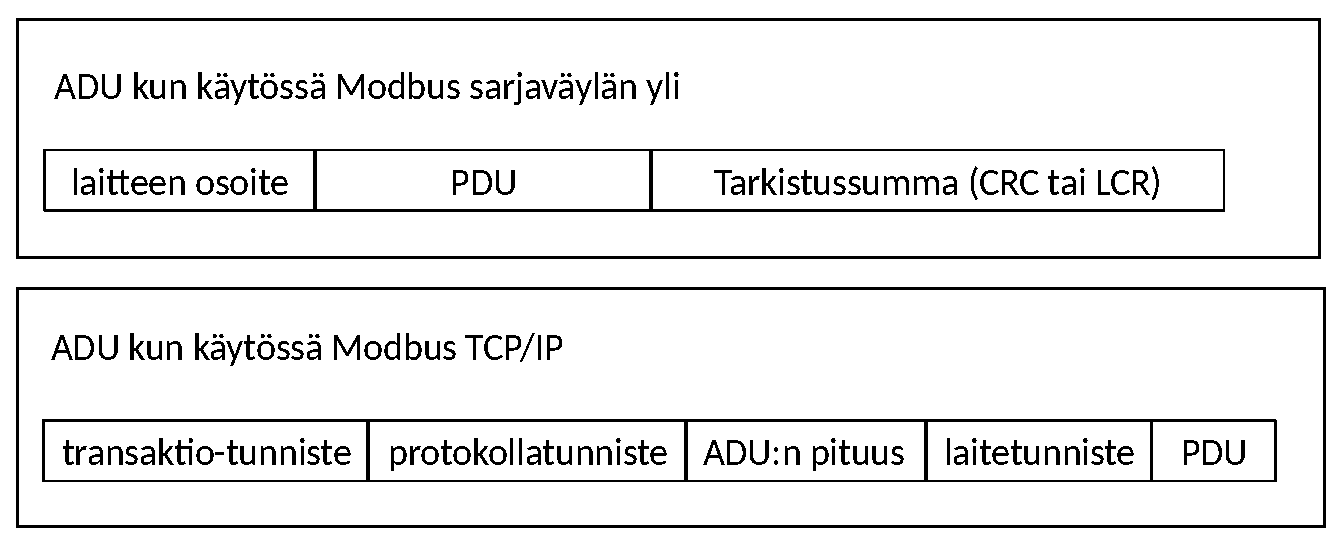
\includegraphics[width=1\textwidth]{figures/adu}
      \caption[ADU-tyypit]{Erilaiset ADU-tyypit.  Perustuen lähteisiin \parencite{modbusTCPIPSpec, modbusSerialSpec}}
      \label{fig:adu}
    \end{figure}

    Sarjaväylän yli toimivassa Modbusissa ADU siirretään käyttäen RS-485-standardia noudattavaa väylää tai RS-232-väylää pitkin. Oletuksena Modbus-standardi kehottaa laitevalmistajia toteuttamaan ainakin RS-485-rajapinnan, RS-232-rajapinnan ollessa vapaaehtoinen. Modbus \gls{RTU} siirtää datan suoraan bitteinä. Modbus \gls{ASCII}:ssa taas jokainen tavu koodataan kahdeksi heksadesimaalimerkiksi ennen lähetystä, mikä heikentää sen tiedonsiirtokykyä. Modbus-standardi edellyttää, että kaikki laitteet tukevat ainakin Modbus RTU:ta Modbus ASCII:n ollessa suositeltu.\parencite{modbusSerialSpec}

    Modbus TCP/IP:tä käytettäessä Modbus-liikenne voi kulkea normaalin Internet-liikenteen mukana, mikä tekee siitä hyvin joustavan ratkaisun. TCP-portti 502 on varattu Modbus-sovelluksille.\parencite{modbusTCPIPSpec} Koska ADU:t lähetetään TCP-kehyksessä, niihin ei tarvitse laskea eikä lisätä tarkistussummaa. TCP-protokolla huolehtii paketin (kehys + ADU) perille pääsystä ja mahdollisista uudelleenlähetyksistä. Tietosuojasta voidaan huolehtia käyttämällä kommunikointiin \gls{VPN}-yhteyttä. Toinen turvallisuutta parantava keino on käyttää kommunikointiin MODBUS/TCP Security -standardin mukaista TLS-salausta, jolloin liikenne kohdistetaan TCP-porttiin 802\parencite{modbusTCPIPTLSSpec}.

\section{IEC 61850}
  \gls{IEC} 61850 on sähköaseman älykkäiden sähkölaitteiden kommunikaatioprotokollia määrittävä standardi. Se on laajasti käytössä sähköasemien tiedonvaihdossa ja sähkönjakelun automaatiossa. Sen laajennukset tähtäävät kuitenkin myös laajempaan käyttöön, sillä standardissa on määritelty myös esimerkiksi hajautetun energiantuotannon tietomalleja. Standardi määrittelee myös inverttereiden erilaisia toiminnallisuuksia, esimerkiksi:
    \begin{itemize}
      \item välittömät ohjaustoiminnot, esimerkiksi alasajo- ja käynnistyskomennot,
      \item loistehonsäädön (Volt/VAR-säätö) tilan muuttaminen,
      \item teho taajuuden funktiona -tilan muuttaminen (frequency-watt),
      \item toiminnan jatkaminen epätavallisista jännitevaihteluista huolimatta,
      \item normaalin toiminta-alueen määrittäminen ja irtikytkeytyminen sen ulkopuolella määritellyllä funktiolla,
      \item käyttäytymistilojen muuttaminen tehon funktiona,
      \item tehon muuttaminen jännitteen perusteella ja
      \item ajastetut komennot \parencite{61850funcs}.
    \end{itemize}

  Vaikka IEC 61850 ei ole vielä laajasti käytössä inverttereissä, esimerkiksi SMA\footnote{SMA Solar Technology AG -- System-, Mess- und Anlagentechnik} tarjoaa Italiassa toimiville inverttereille standardia hyödyntävän rajapinnan \parencite{SMAManual}. Tällä voidaan irrottaa tai kytkeä invertteri verkkoon, tai muuttaa invertterin taajuusrajoja. Italian CEI 0-21 -standardissa vaaditaan inverttereille rajapinta verkonhaltijalle, jonka takia luultavasti tämä ominaisuus on SMA:n ohjekirjassa merkattu vain Italia -ominaisuudeksi. Tämän vaatimuksen\footnote{\url{http://blog.nettedautomation.com/2012/07/iec-61850-in-italy-sma-offers-iec-61850.html}} lähde ei ole alkuperäinen, joten tätä vaatimusta ei voitu vahvistaa varmaksi, tosin SMA:n erillinen ohjeistus Italian laitteille viittaa siihen.


\section{SunSpec Modbus}
  SunSpec Modbus on SunSpec Alliancen määrittelemä sovellustason toteutus, joka hyödyntää yleisesti käytössä olevaa Modbus-protokollaa. Sunspec Modbus sijoittuu rakenteellisesti Modbusin päälle, kuten taulukossa 4.3 kuvattiin. Fyysinen Modbus-rajapinta on sisäänrakennettu noin \SI{80}{\percent}:iin asennetuista hajautetun energiantuotannon laitteista, joten tämän toteutuksen tuominen suurelle määrälle laitteita on melko yksinkertaista \parencite{SSFactSheet}.

  SunSpecin standardi on tehty huomioiden \gls{IEC} 61850 -standardi, mukaan lukien sen 90-7 ja 7-420 -laajennukset, jotka käsittelevät hajautetun energiantuotannon inverttereiden ja konverttereiden toiminnallisuuksia ja kommunikaatiorakennetta hajautetussa energiantuotannossa. SunSpec onkin toteuttanut edellä mainitut toiminnallisuudet myös omaan standardiinsa. Tämän tarkoituksena on helpottaa integraatiota \gls{IEC} 61850 -standardia hyödyntävien järjestelmien kanssa \parencite{SSTech}. Kuitenkaan SunSpec ei ole nimennyt tietomallin muuttujia täsmälleen samoilla nimillä, kuin 61850-standardi, joten ne eivät ole suoraan yhteensopivia keskenään.

  SunSpecin toteutuksessa on määritelty tietomalleja, joiden avulla eri valmistajien laitteita voidaan yhdistää samaan järjestelmään \parencite{SSTech}. Nämä tietomallit mahdollistavat laiteriippumattomuuden, sillä niissä on määritelty funktioiden toiminta ja niiden käyttö. Tällöin eri valmistajien laitteita voidaan lukea ja ohjata yhteisillä käskyillä järjestelmän sisällä.

  SunSpec Modbusin määrittelemät tietomallit ovat käytössä myös muilla protokollilla, kuten \gls{HTTP}/\gls{XML}:lla ja \gls{OPC}:lla \parencite{SSTech}. Koska lähes kaikki tieto SunSpecin standardista perustuu Modbus-protokollaan, muiden tiedonsiirtoprotokollien tarkastelu jätettiin pois. Tiedon puute johtuu mitä luultavimmin Modbusin hallitsevasta asemasta inverttereissä.


\section{IEEE 1815 / Distributed Network Protocol 3}
  DNP3 on teollisuusautomaation kommunikaatioprotokolla, joka määriteltiin alun perin 1993 ja sen kehitys jatkuu edelleen. Vuonna 2008 yhdysvaltalainen valtionvirasto NIST ja voittoa tavoittelematon energia-alan järjestö \gls{EPRI} näkivät tarpeen rajapinnalle \gls{IEC} 61850:n ja DNP3:n välille. Koska DNP3 oli vain vakiintunut käytäntö, DNP3:n standardisointi oli tarpeen, jotta yhteistyö ja koordinointi \gls{IEC}:n kanssa olisi sujuvaa. DNP3 standardoitiinkin \gls{IEEE} 1815 -standardiksi vuonna 2010, jonka jälkeen siitä on käytetty tuota nimitystä \parencite{DNP3&61850}.

  DNP3 on suunnattu sähköteollisuuden käyttöön, mutta se on myös käytössä esimerkiksi energia- ja vesiteollisuudessa. Pohjois-Amerikassa DNP3 on käytössä sähköverkon \gls{SCADA}-järjestelmissä, ja se onkin osittain kilpaileva sähköasemastandardi IEC 61850:n kanssa.

  IEEE 1815.1 -dokumentti määrittelee standardisoidun tavan linkittää yhteen data tämän ja IEC-standardin välillä \parencite{IEEE1815.1}. Tämä mahdollistaa IEC 61850-standardia käyttävien laitteiden lisäyksen IEEE 1815-protokollaiseen järjestelmään. Tämän on Pohjois-Amerikassa tärkeää, sillä siellä on laajasti käytössä IEEE 1815 standardi, mutta koska IEC 61850 on ominaisuuksiltaan laajempi, sen osuus tulee kasvamaan. Molempien standardien kanssa työskentelevä Bruce Muschlitz arveli vuonna 2009 DNP3:n häviävän keskinäisen kilpailun, sillä IEC 61850 täyttää kaikkien sidosryhmien tarpeet ominaisuuksien puolesta \parencite{DNPvsIEC}. Tosin näiden kahden standardin yhteensovittaminen on muuttanut tilannetta, eikä DNP3 tule välttämättä häviämään markkinoilta vielä pitkään aikaan. 2019 tehdyn kyselyn mukaan DNP3:a käytti 94\% kyselyyn vastanneista sähköntuotanto ja -jakeluyrityksistä Pohjois-Amerikassa, mutta IEC 61850:n osuus on kasvamassa \parencite{DNP3Study}.

  Vuonna 2013 DNP3 julkaisi dokumentin, joka auttaa verkonhaltijoita kommunikoimaan hajautetun energiantuotannon kanssa. Tämä dokumentti kuvaa standardoidun rajapinnan datalle ja joukon protokollapalveluita ja profiileja. Dokumentin kuvaamien profiilien tarkoitus on helpottaa hajautetun energiantuotannon liittämistä DNP3 järjestelmiin. Vuonna 2018 dokumenttia päivitettiin siten, että se lisäksi sisältää toiminnallisten ominaisuuden määrittelyt protokollalle, sekä linkityksen IEC-61850-7-420 tietomallin kanssa. Näiden uudistusten myötä DNP3 protokollaa voidaan käyttää älyinverttereiden ohjaukseen samalla tavalla kuin SunSpeciä tai IEC 61850-standardia, mutta myös käyttää näitä kolmea protokollaa rinnakkain toistensa kanssa. \parencite{DNP3Inv, DNP3AppNote}


\section{Smart Grid -ready}

  Bundesverband Wärmepumpe e.V. (jäljenpänä BWP) on saksalainen lämpöpuppuyhdistys, joka ylläpitää lämpöpumppujen ohjaukseen käytettävää rajapintaa määrittävää \gls{SG}-Ready-merkintää (\gls{SG} Ready label). \gls{SG}-Ready määrittelee pumpulle neljä eri toimintatilaa, joiden perusteella ulkoinen toimija kykenee ohjaamaan lämpöpumpun toimintaa. Toimintatilat yksi ja kaksi ovat yhteensopivia Saksassa käytetyn muunmuassa lämpöpumppuihin kohdistetutun energiantoimittajien suorittaman ohjauksen (EVU-Sperre\footnote{Energieversorgungsunternehmen Sperre}) kanssa.\parencite{SGReadyReg} Ohjattava lämpöpumppu voidaan kytkeä energiatoimittajan toimesta pois päältä enimmillään kahdeksi tunniksi kerrallaan. Yhteen vuorokauteen taas voi sijoittua enintään kolme keskeytystä, jotka on pyritään sijoittamaan suurimman kulutuksen hetkiin. Kun kuluttajan tekee sähkösopimuksen, johon ohjaus kuuluu, saa hän vastavuoroisesti alennusta energian hinnasta.\parencite{enwg, VDEARN4100}

  SG-Readyn  kolmas ja neljäs toimintatila ovat sopivia ylituotannon kompensointiin niiden lisätessä lämpöpumppujen sähkönkulutusta. Eri toimintatilat on eritelty taulukossa \ref{sgready}.
  \begin{table}[h]
    \centering
    \caption[\gls{SG}-Ready toimintatilat]{\gls{SG}-Ready toimintatilat. Perustuu lähteeseen \parencite{SGReadyReg}.}
    \begin{tabular}{|c|c|p{3in}|}
      \hline
      \rowcolor{lightgray} toimintatila & looginen kytkentä & kuvaus \\\hline
      1 & 1 0 & Lämpöpumppu on kytkettynä pois päältä. Enintään kaksi tuntia kerrallaan enintään kolme kertaa vuorokaudessa \\\hline
      2 & 0 0 & Normaali toimintatila. Varaudutaan mahdolliseen kahden tunnin pysäytykseen. \\\hline
      3 & 0 1 & Suositeltu päälläolo. \\ \hline
      4 & 1 1 & Pakotettu päälläolo. Mahdollisesti myös lisävastuksen pakotettu päälläolo. \\\hline
    \end{tabular}
    \label{sgready}
  \end{table}
  Jokaiselle toimintatilalle on määritelty binäärinen arvo (0b00 -- 0b11), joka voidaan toteuttaa kahdella loogisella tilalla. SG-Ready ei ota kantaa siihen, miten nämä tilat tuodaan ohjattavalle laitteelle\marginpar{varmista}.\parencite{SGReadyReg}

  SG-Ready on korkean abstraktiotason rajapinta, joka tarjoaa keinoja ohjausrajapintojen yhtenäistämiseen. Alemman tason kommunikointi, johon siis SG-Ready ei ota kantaa, pitää määritellä ja toteuttaa erikseen. Yksi alemman tason kommunikoinnissa yleisesti käytettävä standardi on Modbus-viestintäprotokolla.

\section{AMI-mittari}
  Verkonhaltijan omistamat sähkönkäyttöpaikkojen AMI-mittarit voivat toimia rajapintana lämpöpumpuille, ja tulevaisuudessa ehkä myös aurinkosähköjärjestelmille. Nykyään mittarin mallista riippuen mittareissa voi olla kuormanohjausrele esimerkiksi 2-tariffiohjausta varten, jolloin lämmitys voidaan aktivoida yötariffin alkaessa ja lämmitys tapahtuu halvemmalla hinnalla. Lisäksi Suomessa noin 60\%:ssa sähkönkäyttöpaikoista on etäkatkaisu- ja kytkentäominaisuus, jolla voidaan katkaista sähköt koko sähkönkäyttöpaikasta. \parencite{AMRNykytila}

  Jo asennetuissa mittareissa voi olla luentarajapinta hetkelliselle kulutukselle, mutta se rajoittuu usein vain pulssilähdöksi \parencite{Aidon5510}. Esimerkiksi suomalaisen mittarivalmistaja Aidonin uudemmissa mittareissa on mahdollista lukea dataa \gls{HAN}-rajapinnasta, joka toimii RJ-45 -kaapelin välityksellä. Käytännössä tuo rajapinta käyttää M-bus standardia, ja siitä pystyy lukemaan esimerkiksi virta- ja jännitetietoja sekä tehotietoja verkosta mittarin suuntaan ja mittarista verkon suuntaan. Tätä voidaan hyödyntää kiinteistöautomaatiossa mittaritietona, jolloin asiakas voi kuluttaa kaiken tuottamansa energian sen verkkoon syöttämisen sijaan. \parencite{HAN}

  AMI-mittaria voidaan tulevaisuudessa hyödyntää akullisissa aurinkosähköjärjestelmissä kuormanohjaukseen. Seuraavan sukupolven mittareihin voitaisiin lähettää tieto sähkön hinnasta, jolloin sähkönsyöttöä voidaan vaihtaa verkon ja energianvaraston välillä korkean hinnan aikaan. Älykäs mittarinluentajärjestelmä voi myös hyödyntää historiatietoja ja sääennustusta optimoidessa sähkövaraston käyttöä. Tällöin energiavarastoa voitaisiin varata yöllä halvemman sähkönhinnan aikaan, mutta varaaminen kuitenkin pääsääntöisesti tapahtuisi aurinkovoimalalla. \parencite{AMRNykytila}

  Keskeinen syy mittarien yksinkertaisiin kuormanohjauksiin on mittarin luotettavuus, sillä monimutkaisemmassa mittarissa on useampi hajoava komponentti, ja mittareiden elinkaari on kuitenkin suhteellisen pitkä, 10--15 vuotta. Lisäksi verkonhaltijan saamat hyödyt ylimääräisistä rajapinnoista eivät ole suuret, ja uusien toiminnallisuuksien kehitys myöhäistäisi edelleen seuraavan sukupolven mittareiden asennusta. Lähtökohtaisesti tietoturvan ja kustannusten kannalta kannattavampaa onkin tarjota vain rajapinta mittarilta saatavalle tiedolle, kuten mittaukselle ja esimerkiksi energian hinnalle. Tällöin kiinteistöautomaatio voi hyödyntää näitä tietoja, ja siten hoitaa paikallisesti energiatasapainon optimointia.


\chapter{Sidosryhmät ja niiden tarpeet rajapintojen näkökulmasta}
\label{ch:sidosryhmat}
Luonnollisesti eri sidosryhmät ovat kiinnostuneet erilaisiin käyttötarkoituksiin soveltuvista rajapinnoista. Osa sidosryhmistä on kiinnostunut vain datan lukemiseen tarkoitetusta rajapinnasta käyttäen sitä esimerkiksi käyttövarmuuden ja tuoton tilastointiin, kun taas osa on kiinnostunut järjestelmien etähallinnasta esimerkiksi verkon joustavuuden parantamiseksi. Erityyppisiä sidosryhmiä on hahmoteltu kuvassa \ref{fig:sidosryhmat}, jossa keskellä sijaitsee rajapintoja tarjoavat järjestelmät, vasemmalla sähköverkkoon liittyvät ja oikealla muut sidosryhmät.

\begin{figure}[h]
  \centering
  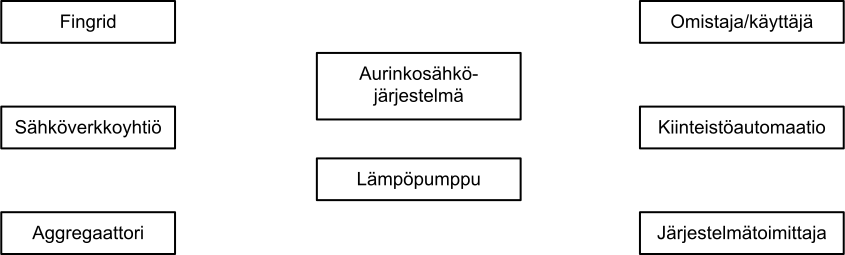
\includegraphics[width=1\textwidth]{figures/sidosryhmat}
  \caption{Järjestelmien sidosryhmiä}
  \label{fig:sidosryhmat}
\end{figure}

\section{Kantaverkkoyhtiö Fingrid}
  Suomen kantaverkkoyhtiönä Fingrid asettaa vaatimuksia siihen liittyen, mitä rajapintoja järjestelmien on sisällettävä. Se vaatii alle \SI{1}{\mega\watt} järjestelmien (voimalaitosten) sisältämään logiikkaportin, jonka kautta saapuvalla käskyllä voimalaitoksen on lopetettava pätötehon tuotanto viiden sekunnin kuluessa. Yli \SI{1}{\mega\watt}:n suuruiset järjestelmät tulee taas varustaa väyläliitännällä, jolla voidaan alentaa tuotannon pätötehoa annetun ohjearvon mukaisesti. Tämän liitännän on oltava yhteensopiva IEC60870-6, IEC60870-5 tai IEC61850 -protokollan kanssa. Fingrid ei dokumentissaan kuitenkaan ilmoita, täytyykö näiden liitäntöjen olla käytössä, vai riittääkö että järjestelmissä on liitäntä olemassa. \parencite{VJV2018}

  Mikäli Fingridin voimajohtoon liitettävä voimalaitos on yli \SI{1}{\mega\watt}:n tehoinen, se on varustettava eroonkytkentäreleistyksellä. Yli \SI{5}{\mega\watt}:n tehoinen voimalaitos vaatii lisäksi eroonkytkennän viestiyhteyden pikajälleenkytkentöjen toiminnan varmistamiseksi. Jos taas voimalaitos liittyy suoraan tai Fingridin asiakkaan verkon kautta kantaverkon kytkinkenttään, ei eroonkytkentäreleistystä vaadita. Tahattoman saarekekäytön estäminen on joissain inverttereissä integroituna, jolloin ne tarkkailevat verkon tilaa ja huomattuaan saarekkeen muodostumisen, kytkeytyvät irti. Tällöin alle \SI{5}{\mega\watt}:n järjestelmät eivät tarvitse erillisiä laitteistoja eroonkytkentään, vaan invertteri toteuttaa itsessään jo tämän vaatimuksen.

  Yli \SI{10}{\mega\watt}:n järjestelmien kohdalla Fingridin kantaverkkokeskus voi tarvittaessa pyytää järjestelmän käytöstä vastaavaa toimijaa muuttamaan pätö- tai loistehosäädön asetteluarvoja voimalaitosteknologian asettamissa rajoissa \parencite{VJV2018}. Fingrid ei täten ota kantaa siihen, miten tämä säätäminen tapahtuu. Fingridin tarpeet järjestelmien rajapinnoista rajoittuvat siten erityistilanteissa järjestelmän alasajoon tai sen tehonsäätöön käytöstä vastaavan toimijan kautta.

\section{Verkonhaltija}

  Yksi järjestelmien rajapintoihin liittyvistä sidosryhmistä on sähköverkonhaltija eli Suomessa sähköverkkoyhtiö. Vuodesta 2009 on Suomessa laki velvoittanut sähköverkkoyhtiöitä asentamaan sähkönkäyttöpaikoille eli pisteisiin, jossa sähköä ostavat asiakkaat liittyvät verkkoon, tuntimittauslaitteiston. Asetus myös asettaa vaatimuksia käytetyllä tuntimittauslaittestolle muun muassa etäluettavuudesta ja -ohjattavuudesta. \parencite{mittariAsetus}

  Älykkäästä tuntimittauslaitteistosta käytetään usein termiä älymittari, \gls{AMR}-mittari tai \gls{AMI}-mittari. Termin \gls{AMR} viitatessa lähinnä mittarin automaattiseen luentaan, saattaisi \gls{AMI}-mittari olla oikeampi termi. Lyhenne \gls{AMI} tarkoittaa mittareiden muodostamaa järjestelmää, jossa tieto liikkuu myös kohti mittareita ja niiden takana olevia kiinteistöjä. \parencite{dictOfEnergy}

  Verkonhaltija ei itsessään ole energian ostaja tai myyjä, vaan se siirtää sähkön verkossa ja on vastuussa verkon toimivuudesta. Tästä syystä verkonhaltijan saamat hyödyt mittareiden etäohjauksesta ovat vähäiset. Yksi hyöty verkonhaltijalle on kuitenkin sähkönkäyttöpaikan irrottaminen verkosta etänä, esimerkiksi laajemman huoltotyön ajaksi. Tällöin verkonhaltijan ei tarvitse käyttää resursseja käydäkseen jokaisessa sähkönkäyttöpaikassa irrottamassa sen sähköverkosta ennen huoltotöitä.

\section{Järjestelmän omistaja}

  Järjestelmän omistajan eli usein käyttäjän suorittama järjestelmän monitorointi voidaan toteuttaa muutamilla eri tavoilla. Monitorointi ja ohjaus toteutetaan usein fyysisen käyttöliittymän avulla ja mikäli nämä toiminnallisuudet halutaan myös etänä, on käyttöliittymä helposti tuotavissa laitevalmistajan tarjoamaan pilvipalveluun tai mobiilisovellukseen. Mikäli valmistaja ei kuitenkaan tarjoa etämonitorointiin sovelluksia, on sellainen usein mahdollista tehdä itse, mikäli osaaminen riittää aiheeseen.

  Omistaja voi olla kiinnostunut myös erilaisista energiaa säästävistä ohjaustoiminnoista, hyvä esimerkki tästä on "poissa kotoa"{} \texttt{-}toiminto, jolla saadaan lämpötilaa laskettua, mikäli kiinteistö on tyhjillään pidemmän aikaa. Tämä luonnollisesti laskee myös lämmityskustannuksia.

\section{Kiinteistö}
  Kiinteistö voidaan ajatella yhtenä sidosryhmänä, joka on hyvin sidoksissa järjestelmän omistajaan.  Tämä johtuu sitä, että omistaja voi ohjata kiinteistöautomaation kautta muitakin laitteita, kuin vain lämpöpumppua tai aurinkosähköjärjestelmää. Tällöin järjestelmä voi säädellä automaattisesti kiinteistön energiatasapainoa, tai siirtää varaavan lämmityksen kulutus halvemmille tunneille.

  Kiinteistöautomaation avulla lämpöpumpun käyntijaksojen aiheuttamaa kiinteistön kuormitusta voidaan kompensoida aurinkosähköinvertterin avulla ja näin vähentää sähkönsiirron kustannuksia sekä parantaa jännitteen laatua heikoissa sähköverkoissa. Automaatiolla voidaan ajoittaa lämpöpumppujen kuormittavin jakso aurinkosähkön tuotantoaikaan, jolloin kiinteistön ottama kuorma verkosta pienenee. Tällä on kiinteistön energiakustannusten kannalta merkitystä erityisesti, jos käytössä on tehotariffi. Tällainen automaatio voi parhaassa tapauksessa mahdollistaa tehotariffissa määritellyn huipputehon pienentämisen kausittain.


\section{Järjestelmätoimittaja}

  Lämpöpumppujärjestelmän tai aurinkosähköjärjestelmän toimittaja voi hyödyntää lämpöpumpun rajapintoja huoltopalveluiden tarjontaan ja diaknostiikkaan. Seuraamalla järjestelmän toimintaa toimittaja voi ennustaa ja tilata tarvittavia huoltoja tai korjauksia, jolloin järjestelmän käyttövarmuus paranee. Tämä tuo käyttäjälle lisäarvoa ja säästöjä sekä huolettomuutta, toimittaja taas voi myydä tämän lisäpalveluna asiakkaalle. Esimerkiksi kuluttajan ei tarvitse käyttää aikaa vikojen selvittämiseen tai huoltojen tilaamiseen. Vastaavasti toimittajan/huoltoyrityksen turhat vierailut vähenevät, kun järjestelmän virhetilanteita voidaan selvittää ja nollata etähallintaa hyödyntäen. Toimittajan suorittamaa diagnostiikkaa voidaan käyttää myös tuotekehityksen apuna tai luotaessa parempia ennustemalleja sähkön kulutuksesta.

\section{Aggregaattori}

  Ennestään sähkömarkkinoilla on ollut käytännössä kolme toimijaa: Energian myyjä, siirtäjä ja ostaja. Aggregaattori näistä kaikista (mahdollisesti) erillinen toimija, jonka tehtävänä on myydä sähkömarkkinoille joustoa. Aggregaattori voi ohjata esimerkiksi lämpöpumppupoolia ja käydä kauppaa sen mahdollistamalla kysyntäjoustolla.

  Lämpöpumput ovat todennäköisesti käyttöpaikkansa suurimpia sähkönkäyttäjiä. Käyttäjän kannalta olisi edullista, mikäli lämpöpumpun käyttämä sähkö hinnoiteltaisiin muusta käytetystä sähköstä erillään. Saksalaisessa EVU-Sparre-järjestelmässä lämpöpumppu on sähköntoimittajan tai muun yrityksen ohjattavissa. Korvauksena kuormanohjauksesta kuluttaja saa hinnanalennusta lämpöpumpun käytetystä energiasta. Tämä tarkoittaa, että energiamittari mittaa erikseen lämpöpumpun käyttämän energian. Myöskin aggregaattorina toimivan yrityksen suorittama ohjaus tapahtuu AMI-mittareiden kuormanohjausreleen kautta. \parencite{enwg, VDEARN4100}

  Vastaavasti aurinkosähköinvertterin ohjaukseen releohjaus ei suoraan sovellu, sillä inverttereiden ohjaus tapahtuu usein monimutkaisemmalla kommunikaatiolla, kuin yksinkertaisella releellä. Sinällään tämä ei haittaa, sillä aurinkosähköjärjestelmän hyödyt etäohjauksen osalta ovat vähäiset; tavoitteena on kuitenkin saada tuotettua mahdollisimman paljon energiaa, ja tämän invertteri hoitaa automaattisesti.

  Mikäli invertterit pystyvät kuitenkin tuottamaan loistehoa pätötehon tuotannosta riippumatta, tästä voi aggregaattori olla kiinnostunut, mikäli niitä voitaisiin ohjata virtuaalivoimalan tavoin isommissa ryhmissä. Nykyisillä ratkaisuilla tällainen ei kuitenkaan ole vielä mahdollista. Esimerkiksi standardoitu rajapinta pilvipalveluintegraatioihin eri valmistajien välillä voisi mahdollistaa tämän.

  Aggregaattori voi myös tulevaisuudessa mahdollisesti ohjata akullisia järjestelmiä virtuaalivoimalan tavoin. Tällöin on sovittava raja-arvot, millaisilla varaustasoilla aggregaattori voi säätää energiavarastoa. Tämäkään ei tosin onnistu releohjauksella, ellei valmistajat sovi yhdessä standardoitua tapaa ohjaukselle.


\chapter{Sovellukset}
\label{ch:sovellukset}
Lämpöpumppujen kommunikaatiorajapintoja voidaan hyödyntää useaan eri tarkoitukseen. Yksittäisten lämpöpumppujen monitorointiin ja hallintaan on olemassa ratkaisuja. Nykyään lämpöpumpputoimittajat saattavatkin tarjoavat lämpöpumpun yhteyteen etäohjauksen mahdollistavia toimintoja ja sovelluksia. Suurempia hyötyjä saadaan kuitenkin useiden useiden yksiköiden muodostamien lämpöpumppupoolien ohjaamisesta. 

Myös aurinkosähköjärjestelmien kommunikaatiorajapintoja voidaan hyödyntää eri tarkoituksiin. Halvimpia malleja lukuunottamatta monet valmistajat tarjoavat suoraan invertterissä etämonitorointimahdollisuuden verkon yli, joillakin on jopa kehitetty mobiilisovellus tätä varten. Lisäksi invertterit tarjoavat usein fyysisen rajapinnan esimerkiksi kodin automaatiojärjestelmään liittämistä varten. 

Tässä kappaleessa käydään läpi erilaisia rajapintoja hyödyntäviä tai niiden mahdollistamia sovelluksia. Sovelluksia käydään läpi nykytekniikan puitteissa, mutta kappaleessa avataan myös tulevaisuudennäkymiä. 


\section{Etämonitorointi ja -ohjaus}

  Ilmeisin tapa hyödyntää lämpöpumppujen kommunikointirajapintoja on etämonitorointi ja -hallinta. Etämonitoroinnilla tarkoitetaan lämpöpumpun toiminnan seuraamista etänä. Seurattavia asioita voivat olla esimerkiksi:
  \begin{itemize}
    \item järjestelmässä kiertävien aineiden ja mahdollisten varaajien lämpötilat,
    \item kompressorin tai sähkövastuksen käyttö,
    \item ulko- ja sisälämpötila,
    \item ja erilaiset hälytykset.
  \end{itemize} \parencite{Latomaki}
  Esimerkiksi lämpöpumpun käyttäjän ollessa poissa kotoa, pystyy hän siitä huolimatta varmistamaan kotinsa lämpötilan ja järjestelmien toimivuuden. Myöskin virhetilanteissa pystytään reagoimaan nopeammin.

  Aurinkosähköjärjestelmän tapauksessa monitorointi tarkoittaa pääosin hetkellisen tuoton ja tuottohistorian tarkastelua. Toki tiedoista enemmän kiinnostunut voi myös tarkastella verkon tilaa invertterin kautta, sillä monissa inverttereissä pystyy jo katsomaan esimerkiksi verkon tehokerrointa sekä taajuutta. Etämonitorointia voidaan hyödyntää myös vikatilanteiden seuraamisessa, esimerkiksi SMA:n Smart Connected -palvelun avulla SMA hoitaa vikatilanteiden viestinnän asiakkaalle, sekä hoitaa oikeiden komponenttien tilaamisen huoltoyritykselle \parencite{SmartConnected}. Tällä tavalla asiakas saa laitteen nopeasti toimintakuntoon, eikä huoltoyrityksen tarvitse käydä ensin paikan päällä tarkistamassa laitetta vaan voi suoraan hoitaa huollon alusta loppuun. 

  Kun lämpöpumppua pystytään monitoroinnin lisäksi myös ohjaamaan etänä, puhutaan etähallinnasta. Toisin kuin pelkästä monitoroinnista, lämpöpumpun etähallinnasta saattaa olla enemmän käytännön hyötyä myös omakotitaloasujalle. Etähallinnalla voidaan saavuttaa energian säästöä eri tavoilla. Etähallinta mahdollistaa muunmuassa matalamman sisälämpötilan ylläpitämisen asukkaiden ollessa poissa, minkä jälkeen voidaan nostaa asunnon lämpötilaa juuri ennen asukkaiden paluuta kotiin. Kesällä sama periaate pätee jäähdytykseen, mikäli käytettävä lämpöpumppu toimii myös jäähdyttävänä järjestelmänä. Tälläistä saatetaan kutsua esimerkiksi lomatoiminnoksi. Etähallintasovelluksesta on myöskin helppo tehdä intuitiivinen käyttää, koska käyttöliittymä voidaan tuoda kiinteästi lämpöpumpun yhteyteen asennetuista sulautetuista käyttöliittymistä käyttäjän omalle laitteelle.

  Aurinkosähköjärjestelmän etähallinnalla ei kotitalouksissa ole tarvetta, sillä järjestelmä on suunniteltu toimimaan jatkuvasti parhaalla tuotolla. Etähallinnasta voi tosin olla kiinnostunut tulevaisuudessa verkonhaltija, sillä se voi tällöin rajoittaa maksimitehoa tai muuttaa esimerkiksi sen käyttäytymistä eri jännite- tai taajuusalueilla. Lisäksi se voi pakottaa koko järjestelmän pysäyttämisen. Tällä hetkellä verkonhaltijan etäkäytön estää oikeastaan puuttuvat järjestelmäintegraatiot, sillä nykyisiin energiamittareihin ei ole integroitu kommunikaatiota ulkoisille laitteille. Aurinkoinverttereiden integrointi verkonhaltijan \gls{SCADA}-järjestelmään on toki mahdollista, mutta se on järkevää vain suuremmissa järjestelmissä nykyisillä standardeilla, sillä verkonhaltijalla ei ole kaksisuuntaista kommunikaatiota kotitalouksiin ennestään. 

  Kommunikointi lämpöpumpun ja asiakkaan päätelaitteen, joka voi olla esimerkiksi puhelin tai tietokone, voi tapahtua monella erilaisella tavalla. Monet lämpöpumppuvalmistajat tarjoavat lämpöpumppuihinsa lisäpalveluna etäohjaustoiminnallisuutta, joka näyttäytyy käyttäjälle esimerkiksi mobiilisovelluksena tai selaimessa käytettävänä verkkosovelluksena. Lämpöpumpputoimittajan tarjoamissa ratkaisuissa ei vaadita käyttäjältä yleensä sen suuryttäjälle esimerkiksi mobiilisovelluksena tai selaimessa käytettävänä verkkosovelluksena. Lämpöpumpputoimittajan tarjoamissa ratkaisuissa ei vaadita käyttäjältä yleensä sen suurempaa perehtymistä tai asiantuntemusta. Toimittaja saattaa myös tarjota valmiita ratkaisuja lämpöpumpun integroimiseen taloautomaation kanssa.

  Lämpöpumpun etäohjaus voidaan toteuttaa myös itse, mikä vaatii käyttäjältä enemmän asiantuntemusta. Tällöin pitää ohjattavan lämpöpumpun tarjota jokin ohjausrajapinta, esimerkiksi modBUS-väylä tai vastaava, tai vähintäänkin lämpöpumpun pitää tukea tämän mahdollistavaa laajennusta. Käyttäjän pitää itse toteuttaa ainakin ohjauslogiikka, käyttöliittymä ja päättää minkälaista palvelinta haluaa ylläpitää näiden mahdollistamiseksi.

  Yksittäisen lämpöpumpun ohjauksella saavutettavat hyödyt ovat lähinnä yksittäisen omakotitalokäyttäjän saavuttamia säästöjä tai vastaavasti teollisuudessa tapahtuvaa järjestelmien hallinnasta saavutettavia etuja. Merkittävämmät lämpöpumppujen rajapintoja hyödyntävät sovellukset koskevat hyödyt saavutetaan, kun ohjattavia lämpöpumppuja on useampia.

\section{kysyntäjousto}

  Normaalissa keskitetyssä sähköenergiajärjestelmässä sähkötehon kulutus vaihtelee muunmuassa vuodenajan, vuorokaudenajan ja sään mukaan. Valmistava suurteollisuus, eli metsä-, metalli- ja kemianteollisuus, kuluttaa noin \SI{40}{\percent} Suomessa käytetystä sähköstä Tästä johtuen teollisuuden prosessien tila saattaa vaikuttaa merkittävästi järjestelmän tehonkulutukseen\parencite{SVTehk}. Sähköverkosta otetun ja siihen syötetyn tehon pitää jatkuvasti olla yhtä suuret, minkä takia tuotantotehoa pitää säätää. Perinteisessä järjestelmässä tehonkulutuksen muutoksia ennakoidaan ja tehontuotantoa säädellään ajamalla esimerkiksi lauhde- ja \gls{CHP}-voimaloita tietyn suunnitelman mukaan.\parencite{energiateollisuus} Niin kutsutut pohjavoimalaitokset, kuten esimerkiksi ydinvoimalaitokset ja osa \gls{CHP}-voimaloista taas ajavat käytännössä koko ajan nimellistehollaan tuottaen suurimman osan kulutetusta energiasta. Vuonna 2018 ydinvoimalla ja CHP-voimaloilla tuotettiin noin \SI{44}{\tera\watt\hour} sähköä, mikä vastaa hieman alle puolta Suomen vuotuisesta sähköenergiantuotannosta.\parencite{SVTSaLaTuo} Pohjavoimalaitoksille tyypillistä on polttoaineen suhteellisen halpa hinta, ja täten kohtuulliset muuttuvat kustannukset investointikustannusten ollessa niihin verrattuna suuria. Myöskin uusiutuvaa energiaa, kuten tuuli- ja aurinkovoimaa ajetaan käytännössä myös jatkuvasti nimellistehollaan, sillä polttoainekustannuksia ei ole.

  Vaikka lauhdevoimalaitoksia käytetään osaltaan säätötehona, niitä ei kannata kuitenkaan käyttää tehonkulutuksen lyhytaikaisten vaihteluiden kattamiseen. Normaalissa laudevoimalaitoksessa esimerkiksi käynnistysajat ovat niin pitkiä, että sekuntitasolla tapahtuva tuotannon lisäys ei onnistu.\parencite{VJV2018} Suomessa yleisesti ja erityisesti sekuntitasolla tapahtuva tehotasapainon säätö tapahtuu pääosin vesivoimalla\parencite{energiateollisuus}, sillä vesimvoiman tehontuottoa kyetään säätämään lähes reaaliajassa säätelemällä veden virtausta turbiineille. Sähköenergiajärejestelmässä esiintyvä tehoepätasapaino aiheuttaa muutoksia jännitteen taajuuteen. Ylituotannon aikana voimaloiden geeraattoreiden pyörimistä vastustava momentti pienenee, jolloin pyörimisnopeus ja täten jännitteen taajuus pääsee kasvamaan. Alituotannon kohdalla tilanne on päinvastainen. Jännitteen taajuutta seuraamalla kyetään ohjaamaan säätövoiman tuotantoa lähes reaaliajassa. Kantaverkkoyhtiö Fingrid myöskin edellyttää voimalaitoksilta taajuusohjattua häiriöreserviä, joka on kyettävä ottamaan käyttöön, mikäli sähköverkon taajuus eroaa \SI{0.5}{\hertz} tai enemmän nimellistaajuudesta \SI{50}{\hertz} \parencite{VJV2018}.

  Uusiutuvien energialähteden käyttö sähköntuotannossa tuo omat haasteensa tehotasapainon ylläpitoon. Eniten käytettyjen uusiutuvien energialähteiden, eli aurinko- ja tuulivoiman, tuotanto riippuu voimakkaasti säästä ja vuorokaudenajasta. Kasvava vaihtelevien energialähteiden käyttö luo entisestään tarvetta säätövoimalle.\parencite{energiateollisuus} Säätövoima on kuitenkin huomattavasti kalliimpaa kuin pohjavoima. Kulutushuippujen aikana käytettävien huippuvoimalaitosten polttoainekulut ovat suuret, niiden käyttäessä sähköntuotantoon esimerkiki maakaasua tai hiiltä. Säätövoimaksi hyvin soveltuvaa vesivoimaa ei myöskään ole tarjolla määrättömästi. Sähköenergian varastointia ei nähdä vielä ratkaisuna uusiutuvan sähköntuotannon vaihteluihin. Monesta tekijästä johtuen sähkön tuotanto on muuttumassa vähemmän joustavaksi.

  Yksi tapa ratkaista sähköntuotannon joustamattomuuden aiheuttamia engelmia on kysyntäjousto, jossa tuotannon sijasta säädellään sähkön kulutusta reaaliajassa, etukäteen tehdyn suunnitelman mukaan tai ohjaamalla kuluttajaa tiettyihin valintoihin. Kysyntäjoustoa voidaan toteuttaa monella tapaa.\parencite{fingrid} Yksi tapa on ohjata sähkön kulutusta hinnoittelun avulla. Tuntihinnoitellun sähkön hintaa kuluttajalle säädellään tuotannon ja kulutuksen mukaan, suurimman hinnan osuessa suurimman kulutuksen ajalle. Äärimmäisin esimerkki kulutusjoustosta on kantaverkkoyhtiö Fingridin toteuttama sähkön kulutuksen alentaminen katkaisemalla jännite tietyiltä alueilta. Viimeisenä mainittua kulutuksen rajoittamista ei kuitenkaan tarvita, mikäli sähköverkossa ei ole suurta vikaa.

  Sähköverkossa olevilla suurilla yhtenäisillä kuormilla, joiden kulutusta pystytään ohjaamaan, voidaan toteuttaa kysyntäjoustoa\parencite{fingrid}. Suomessa on käytössä noin miljoona (vuonna 2019) lämpöpumppua\parencite{sulpu}. Mikäli lämöpumpun keskimääräiseksi sähkötehoksi käytön aikana arvioidaan esimerkiksi \SI{1}{\kilo\watt}, tulee niiden yhteistehoksi \SI{1}{\giga\watt}. Tämä vastaa noin yhtä neljästoista koko Suomen sähkökulutuksesta kovimman sähkönkulutuksen aikaan. Suurimman lämmitystehontarpeen aikana saatetaan myöskin käyttää lämpöpumpun yhteyteen asennettua lisälämmitysvastusta, jolloin yksittäisen lämpöpumpun sähköteho nousee selvästi.

\subsection{Virtuaalivoimalat}

  Virtuaalivoimala on yksi tapa toteuttaa kysyntäjoustoa. Virtuaalivoimala koostuu pienistä sähköä tuottavista yksiköistä tai yhdestä tai useammasta kuormasta, joiden tehonkulutusta ohjataan yhtenä yksikkönä. Virtaalivoimalan omistaja myy sähkömarkkinoille joustokapasiteettia. Suuren sähkönkulutuksen aikana kantaverkkoyhtiö maksaa virtuaalivoimalaoperaattorille siitä, että voimalaan kuuluvissa kiinteistöissä tai muissa kulutuskohteissa vähennetään sähkön käyttöä hetkellisesti. Vastaavasti ylituotantotilanteessa kantaverkkoyhtiö voi ostaa virtuaalivoimalalta kulutusta vastaamaan sen hetkistä tuotantoa. Reservimarkkinoiden hinnat siis määrävät virtuaalivoimalasta saatavan taloudellisen hyödyn. Ostamaansa joustokapasiteettia kantaverkkoyhtiö Fingrid käyttää sähköenergiajärjestelmän tehotasapainon hallintaan. Virtuaalivoimalan ohjaus tapahtuu automaattisesti ja sitä voidaan ohjata esimerkiksi sähköverkon taajuuden mukaan.\parencite{fingrid}

  Osa virtaaalivoimalan ympäristömerkityksestä koostuu siitä, ettei erillistä sähköntuotantolaitteistoa tarvitse rakentaa, vaan toiminta perustuu olemassa olevan tai tarpeeseen rakennettavan laitteiston lisähyödyntämiseen. Mikäli virtuaalivoimala koostuu kulutustaan vähentävistä yksiköistä, ei fingridin voimalaitoksille tarkoitetut verkkoonliittymismääräykset ole päteviä\parencite{VJV2018}.

  Virtuaalivoimala voidaan koostaa kohteista, joissa energiaa saadaan varastoitua väliaikaisesti. Energiaa voidaan varastoida käyttökohteessa esimerkiksi akkuihin, josta esimerkkinä toimii kauppakeskus Sellon virtuaalivoimala Espoossa\parencite{sello}. Myöskin sähköautojen akkuja voidaan käyttää energian varastointiin, tällöin puhutään \gls{V2G}-tekniikasta\parencite{dictOfEnergy}. Mikäli energiaa varastoidaan itsenäisesti toimivaan suureen akustoon, tai esimerkiksi paineilmavoimalaitokseen tai pumppuvoimalaitokseen, puhutaan silloin yleensä sähköenergian varastoinnista, eikä virtuaalivoimalasta\parencite{dictOfEnergy}. Lämpöpumpuista koostuvalle virtuaalivoimalalle ominaista on siis nimenomaan kulutusjouston myyminen, ei niinkään energian.

  Energiaa saadaan varastoitua lämmitysjärjestelmiin. Virtuaalivoimalan toimiessa osana lämmitysjärjestelmää, käytetään esimerkiksi lämminvesivaraajaa, sisäilmaa tai kiinteistöä itseään energiavarastona. Kun Virtuaalivoimalaa käytetään kompensoimaan alituotantoa, kytketään lämpöpumppu, lämmitysvastus tai muu vastaava sähköä kuluttava toiminta pois päältä. Lämmityslaitteiden poiskytkemisaika on yleensä maksimissaa muutamia tunteja, minkä ansiosta lämmitettävä kiinteistö tai kohde ei ehdi jäähtymään merkittävästi, eikä esimerkiksi asumismukavuudesta tarvitse tinkiä. Kun taas kompensoidaan ylituotantoa, voidaan esimerkiksi lämpöpumppuja käyttää maksimitehollaan, kunnes lämminvesivaraaja, kiertovesi tai sisäilma saavuttaa asetetun maksimilämpötilansa. Lämpöpuppujen kompressoreiden lisäksi myös lisälämmitysvastuksia voidaan käyttää, jolloin käytetty sähköteho saatta olla jopa kaksinkertainen.

\subsection{Huipputehon rajoittaminen}

  Osa sähköenergiajärjestelmän kuluista ja päästöistä aiheutuu siirtoverkon rakentamisesta ja ylläpidosta. Rakennettaessa uutta yhteyttä, mitoitetaan sen kuormitettavuus eli sähkönsiirtokyky arvioidun mahdollisen huipputehon mukaan. Suurimman osan ajasta siirtojohdot ovat siis kuormitettuina huomattavasti mitoitustaan pienemmällä kuormalla.\marginpar{sähköverkot-kirja lähteeksi}

  Rajoittamalla johdolla syötetyn alueen huipputehoja, saatetaan välttää uusien yhteyksien rakentaminen. Siirtojohdolla tapahtuvat jännitehäviöt ovat myös suurimmillaan suurimman tehonkulutuksen aikana, joten rajoittamalla huipputehoja, pystytään alentamaan johdolla tapahtuvia häviöitä.

  Sopivan lämpöpumppupoolin ohjauksella voidaan alentaa muuntopiirin tai syötetyn alueen huipputehoa. Riippuen alueesta, lämpöpumput ovat hyvä valinta ohjattavaksi kuormaksi. Uusilla rakennettavilla asuinaueilla, missä kaukolämpö ei ole käytössä, on todennäköisesti suurimmassa osassa asuinrakennuksia lämpöpumppu. Myöskin vanhaa rakennuskantaa peruskorjattaessa lämpöpumput valitaan usein lämmitysjärjestelmän osaksi. Normaalissa omakotitalossa lämpöpumppu on todennäköisesti suurin yksittäinen sähköä kuluttava laite, mikä tekee siitä edelleen hyvän valinnan ohjattavaksi kuormaksi.

  Lämpöpumppupoolin ohjuksesta on myös hyötyä hieman pidemmän sähkökatkon yhteydessä. Sähkökatkon kestäessä hieman pidempään, kylmenevät lämpöpumppujen lämmittämät kohteet. Näin ollen sähköjen palatessa, käytännössä kaikki muuntopiirin lämpöpumput käynnistyvät samaan aikaan. Mikäli kaikki tai osa lämpöpumpuista on varustettu suoraan verkkojännitteeseen kytketyllä oikosulkumoottorilla, voi niiden yhteenlaskettu käynnistysvirtapiikin aikainen tehon kulutus olla huomattavan korkea. Mikäli lämpöpumppujen rajapinnat mahdollistavat yksittäisten lämpöpumppujen ohjaamisen keskitetysti, voidaan sähköjen takaisinkytkeytymisen aiheuttamaan kulutuspiikkiä tasoittaa.

  Voidaan myös ajatella, etteivät lämpöpumput ole kaikkein kriittisimpiä syötettviä kohteita. Mikäli sähköpulan takia on tarpeen rajoittaa kulutusta, on hyvä, jos kuitenkin pystytään takaamaan kriittiset toiminnot, kuten valaistus, kunnallistekniikan toiminta tai kylmälaitteiden käynti. Suomessa useimmissa omakotitaloissa on kuitenkin edelleen tulisija, jolloin lämpöpumppujen jatkuva päälläolo ei ole välttämätöntä lyhyillä, muutaman vuorokauden aikaväleillä. Mikäli sähköpulan aikana voidaan keskitetysti rajoittaa lämpöpuppujen käyttöä, saateetaan vähentää tarvetta alueiden kokonaan jännitteettömiksi kytkemiseen.

\section{Aurinkosähkön kustannustehokas hyödyntäminen}

  Tällä hetkellä aurinkosähkön myynti ei ole kotitalouksissa kannattavaa. Tämän vuoksi tärkeää olisikin käyttää kaikki tuotettu energia itse, jolloin siitä saatu rahallinen hyöty olisi mahdollisimman suuri ja siten takaisinmaksuaika lyhyempi, kuin ylijäämäsähköä myymällä. Tähän voidaan hyödyntää aurinkoinvertterin ja lämpöpumpun kommunikaatiorajapintoja.

  Monissa inverttereissä on mahdollista ohjata erilaisia kuormanohjausreleitä ohjaussignaaleilla. Tällaisia ohjausmahdollisuuksia ei kuitenkaan usein ole suoraan invertterissä, vaan ne on toteutettu modulaarisena komponenttina, joka voidaan ostaa ja asentaa invertteriin erikseen. Ohjaussignaaleita voidaan antaa eri kriteereillä, esimerkiksi aktivoida signaali määrätyn tuottotehon ylittyessä ja deaktivoida se, kun tietty tehotaso alittuu. Tällä tavalla voidaan ohjata esimerkiksi lämpöpumppua tai lämminvesivaraajan vastusta, jotta sähkö saadaan varastoitua lämpöenergiana.

  Aurinkoinvertterissä ei itsessään kuitenkaan ole reaaliaikaista energiamittausta, eikä nykyisissä verkonhaltijan energiamittareissa ole reaaliaikasta mittausta, jota invertteri tai kodin automaatiojärjestelmä voisi hyödyntää. Reaaliaikanen mittaus saadaan erillisellä energiamittarilla, tai tulevaisuudessa seuraavan sukupolven AMI-mittareilla. Reaaliaikainen mittaus mahdollistaa sähkön nettomittauksen, jolloin esimerkiksi varaajasta voidaan aktivoida vain sen vaiheen lämmitysvastus, joka meinaa siirtää sähköä verkkoon päin.

  \section{Mahdolliset haittavaikutukset}

  Rajapinnat ja niitä hyödyntävät sovellukset tuovat haasteita ja mahdollisia haittavaikutuksia. Kuten monesti uuden tekniikan käyttöönottoon liittyy, turvallisuusnäkökulma saattaa jäädä aluksi huomioimatta. Osa haittavaikutuksista saattaa taas ilmetä vasta testattaessa tekniikoita käytännössä tai kun niiden käyttö alkaa olemaan laajalle levinnyttä.

  Lämpöpumppuja kytketään verkkoon, jotta käyttäjät voivat etäohjata sitä tai jotta sitä voidaan ohjata agregaattorin toimesta osana lämpöpumppupoolia. Erään riskityypin muodostavat vahingosa tai huolimattomuuttaan avoimeksi jätetyt ohjausrajapinnat. TCP-portteja voi olla avoinna niin, että kolmas osapuoli voi koittaa avata telnet- tai ssh-yhteyksiä laitteeseen. Mikäli yhteyden saa avattua käyttäen vakiokäyttäjätunnuksia ja -salasanoja,  tai mahdollisesti täysin ilman tunnistautumista, ovat laitteet käytännössä kenen tahansa käytettävissä. Mikäli laitteisiin otetaan yhteyttä salaamattomilla protokollilla, voidaan ohjausliikenteestä urkkia tietoja, joiden päätytminen ulkopuolisten korviin ei ole hyvä juttu. Mahdollisia urkittavia asioita voi olla esimerkiksi asukkaan läsnäolo tai tieto peseytymisajoista, joiden vuotaminen ulkopuolisille voi vaikuttaa vähintääkin turvallisuudentunteeseen.

  Kaapattujen eli luvatta etäohjattujen laitteiden väärinkäyttöön on monia tapoja. Pumppujen voidaan esimerkiksi ohjata tuottamaan omistajilleen ylimääräisiä kuluja tai vaihtamaan asunnon lämpötila täysin vääräksi. Mikäli lämpöpumpun yhteydessä on sulautettuna järjestelmänä esimerkiksi jokin linux- tai windows-käyttöjärjestelmä ohjaamassa pumpun toimintaa, pätevät siihen samat uhkakuvat kuin normaalin kotitietokoneen haltuunnottamiseen. Mikäli kolmas osapuoli kykenee asentamaan lämpöpumppua ohjaavaan tietokoneeseen omia ohjelmiaan, sitä voidaan käyttää vahingollisiin tarkoituksiin esimerkiksi hajautetun palvelunestohyökkäyksen toteuttamisessa. Mikäli kolmannella osapuolella on mahdollisuus käyttää useampaa laitetta yhtäaikaa voidaa laitteita käyttää esimerkiksi häiriöiden tuottamiseen sähköverkossa, eli tuottamaan lisää niitä ongelmia, joiden ratkaisemiseen rajapintojen hyödyntämisellä pyritään.

  Ihmisen turvalisuuden tunnetta lisää, kun hänellä on tunne siitä, että asioita voi kontrolloida itse. Kun Lämpöpumpun ohjausta halutaan siirtää älykkäässä sähköverkossa kolmansille osapuolille kuten agregaattoreille, tämä turvallisuuden tunne saattaa horjua.


\chapter{Yhteenveto}
\label{ch:yhteenveto}
Lämpöpumppujen ja aurinkosähköjärjestelmien merkitys sähköverkossa kasvaa niiden suosion kasvaessa. Lämpöpumput korvaavat muita lämmitys- ja viilennysmuotoja ja aurinkosähköjärjestelmillä haetaan kotitalouksissa omavaraisuutta ja ylipäätään säästöjä sähkölaskussa.

Aurinkosähköjärjestelmien määrän kasvu lisää sähköverkon tuotannon ailahtelevuutta ja säätövoiman tarvetta, sillä tuotanto vaihtelee tunneittain. Tuotantoa voidaan ennustaa sääennusteen pohjalta, mutta yksittäiset pilvet voivat aiheuttaa alueellisesti nopeitakin tehovaihteluita. Lisäksi huipputeho sijoittuu päiväsaikaan, joten ihmisten palatessa töistä ja kulutuksen kasvaessa tuotannon laskiessa samanaikaisesti säätötehon tarve kasvaa entisestään.

Lämpöpumppujen lisääntyminen ja esimerkiksi suorasta sähkölämmityksestä eroava käyttäytyminen vaikuttavat sähköverkkoon. Lämpöpumppujen tekniikka kehittyy ja nykyisin kotitalouskäyttöön myytävissä pumpuissa on yleensä suoraan verkkoon kytketyn oikosulkumoottorin tilalla taajuusmuuttajakäyttöinen oikosulkumoottori. Tämä kehitys myös osaltaan määrittelee miten verkkoon liitettyjen lämpöpumppujen määrän kasvu vaikuttaa sähköverkkoon. Ilman taajuusmuuttajaa tai pehmokäynnistintä verkkoon kytketyt lämpöpumput ottavat käynnistyessään verkosta suuria hetkellisiä tehoja, mikä saattaa jännitejäykkyydeltään huonossa verkossa aiheuttaa hetkellisiä jännitteenalenemia. Lämpöpumpun ollessa taajuusmuuttajakäyttöinen, ei se aiheuta edellä mainittuja tehonkulutuksen piikkejä. Kuitenkin mikäli lämpöpumpulla korvataan jokin muu lämmitysmuoto, kuin suora sähkölämmitys, kasvattaa se kulutuspaikan sähköenergian kulutusta. Mikäli muuntopiirissä moni talous vaihtaa lämmitysmuodokseen lämpöpumpun, saattaa se aiheuttaa tarpeen sähköverkon jännitejäykkyyden parantamiselle.

Järjestelmien tuomia haasteita voidaan ratkaista ja löytää uusia järjestelmiä hyödyntäviä sovelluksia, kun kommunikaatio niiden kanssa mahdollista. Kommunikointi mahdollistetaan standardoiduilla kommunikaatiorajapinnoilla, joiden kautta järjestelmiä voidaan ohjata. Tällöin ne voidaan kytkeä esimerkiksi kiinteistöautomaatioon tai muuhun ulkoiseen ohjaukseen. Valmistajien suljetut pilvipalvelut muodostavat myös erään rajapinnan kommunikaatiolle, joihin pääsy on usein vain valmistajalla ja järjestelmän omistajalla.

Yksi suosituimmista järjestelmien ohjauksen mahdollistavista tekniikoista on Modbus. Modbus-standardi määrittelee fyysisen tason rajapinnat mahdollistaen ohjauksen joko sarja- tai Ethernet-liitäntää käyttäen, mikä mahdollistaa protokollan käyttämisen paikallisesti tai internetin yli toimivien etäyhteyksien välityksellä. Modbus-standardin määritellessä kommunikointia vain hyvin matalalla tasolla on sitä helppo soveltaa erilaisiin sovelluksiin ja sen päälle voidaan rakentaa korkeamman tason viestintä- ja ohjausprotokollia. Modbusin päälle voidaan myöskin toteuttaa yksittäisen laitteen ohjaukseen ja monitorointiin tarvittavat sovellukset tai liittäminen kotiautomaatioon osaksi älykästä kotia.

Aurinkosähköjärjestelmien ja energiavarastojen osalta työssä tarkasteltiin muutamia eri rajapintoja, joista tärkein on SunSpec Modbus. Se pohjautuu Modbus-standardiin, ja sen avulla voidaan ohjata energiavarastojen ja aurinkosähköinverttereiden toimintaa, esimerkiksi rajoittaa tehoa tai säätää loistehontuotantoa. Suurin käyttö tällä rajapinnalla on paikallisessa automaatiossa, esimerkiksi tuotantotietojen käyttö kuormanohjaukseen.

Lämpöpumppujen kohdalla korkeamman tason rajapintoja kuten SG-Ready-ohjausrajapintaa tai Saksalaista EVU-Sperre-ohjausrajapintaa käyttävät sovellukset taas keskittyvät yhden lämpöpumpun sijasta useamman pumpun muodostamaan pooliin. Lämpöpumppupoolin ohjaamista voidaan käyttää erilaisiin sovelluksiin kuten huipputehon rajoittamiseen verkossa tai sähköntuotannon ja -kulutuksen tasapainottamiseen. Aggregaattorin hallinnoimaa lämpöpumppupoolia voidaan käyttää esimerkiksi kysyntäjouston tehokkaaseen toteuttamiseen. Aggregaattorille lämpöpumppupoolin ohjaaminen taas on pääasiallista liiketoimintaa, jolla se osallistuu sähkömarkkinoille.

Työssä tarkasteltiin kuutta eri sidosryhmää, joista Fingrid on sidoksissa vain aurinkosähköjärjestelmiin. Muut sidosryhmät hyödyntävät eri kommunikaatiorajapintoja eri tarkoituksiin, joista osalle niiden käyttö voi olla myös yrityksen ydinliiketoimintaa.

Rajapinnat mahdollistavat useita sovelluksia, mutta kaikki käsitellyt sovellukset eivät vielä ole yleistyneet Suomessa. Etämonitorointi ja -hallinta on ollut jo pidempään käytössä pilvipalveluiden muodossa, ja kiinteistöautomaatio yleistyy kotitalouksissa energiansäästötarkoituksessa.

Kysyntäjousto on vasta yleistymässä Suomessa, sillä aggregaattoreita ei Suomessa oikeastaan ole. Itsenäisen aggregaattorin laajennettu pilotti käynnistyi 21.7.2020, ja siinä testataan aiemmin kokeiltujen ratkaisujen skaalautuvuutta. Fingrid on ajamassa tätä kaikille säätösähkömarkkinoille avointa pilottia eteenpäin.

Teollisuuslaitosten tarvitsemia loistehon kompensaattoreita voidaan tulevaisuudessa korvata aurinkosähköjärjestelmillä, sillä suuritehoiset invertterit voivat tuottaa nimellistehollaan myös loistehoa ympäri vuorokauden. Tällöin kalliiden loistehon kompensaattoreiden takaisinmaksuaikaa voidaan pienentää, kun sitä voidaan hyödyntää myös sähköntuotantoon.

Kommunikaatiorajapintojen hyödyntäminen vaatii vahvaa standardointia, jotta järjestelmät olisivat valmistajasta riippumattomia. Järjestelmien fyysisten rajapintojen osalta tämä alkaa olla jo hyvällä mallilla, mutta niiden hyödyntäminen vaatii vielä kehittämistä. Vielä on kysymysmerkkinä, miten esimerkiksi Suomessa aggregaattori voi ohjata poolina akullisia aurinkosähköjärjestelmiä, tai mitä rajapintaa se käyttäisi virtuaalivoimalaitoksen kautta yksittäisten lämpöpumppujen ohjaamiseen.


\printbibliography[heading=bibintoc]


\begin{appendices}

\chapter{Modbus funktiokoodit}
\label{app:modbus_funktio_koodit}
\begin{figure}[h]
  \centering
  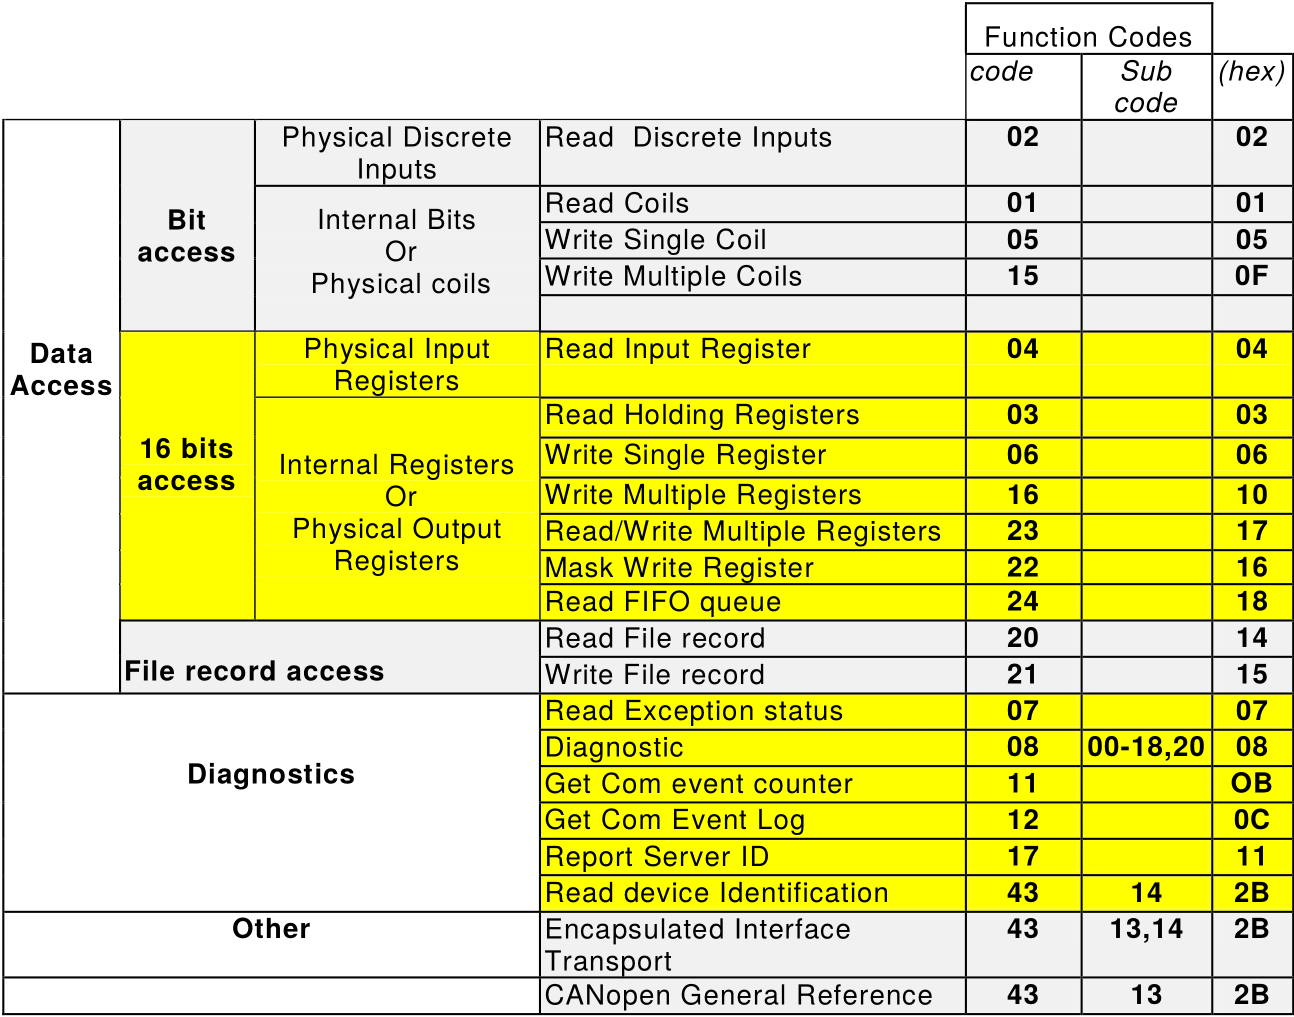
\includegraphics[width=1\textwidth]{figures/modbus_funktio_koodit}
  \caption[Modbus funktiokoodit]{Modbus funktiokoodit. Perustuen lähteeseen \parencite{modbusAppSpec}}
\end{figure}


\end{appendices}

\end{document}
